\chapter{Compiler Overview}\label{Chp:CompilerOverview}
When creating a compiler there is two basic ways of compilers one can create, a multi-pass compiler or a single-pass compiler.
Each have their advantages and disadvantages however the most significant difference is that in a single-pass compiler, as the name suggests, only one pass is done.
This highly limits the information available to the compiler and this decreases the odds of creating efficient programs, which is not wished for in \gls{gamble}.
As such this compiler will be a multi-pass compiler, such a compiler can be divided into phases.
In this chapter the different phases of the compiler and their goals and tasks will be presented, to give an overview for the chapters to come.

The compiler for \gls{gamble} is separated into three phases: syntax analysis, contextual analysis and code generation.
\myref{fig:phases} shows a state diagram of the phases of the compiler.
Syntax analysis and contextual analysis transforms the source code into an intermediate representation, and verifies the source code according to the specified syntax from the \acrshort{cfg}, and also for type and scope checking.
The choice of language for writing the compiler falls upon Java 1.8, which is used in the language and compiler course.
When making a compiler an object-oriented language simplifies many tasks, because of encapsulation, polymorphism and inheritance. 
The paradigm allows for many structural options, and reuse of code when inheriting, which would be impossible using another paradigm like imperative or functional programming.
Java also works across platforms, which is a useful feature.

In the syntax analysis phase the input source code is parsed and separated into tokens according to the \acrshort{cfg}.
This is the scanner's job, the parser structures these tokens into a tree structure, which can be traversed in the order of the source code.
When the source code has been parsed the tree is then simplified to remove unnecessary information such that a tree with less nodes is to be traversed.

In the contextual analysis phase the tree is used to generate a table, containing all the variables and functions which is declared in the source code.
This is called a symbol table, and it is used to check if the variables and functions called and used in the source code are in scope, and also if they uphold the type rules of \gls{gamble}.
This phase results in telling the programmer if a mistake is found in the source code and where the mistake is located, and also what is wrong, but it also results in the tree now containing additional information about the type of expressions in the source code.

The last phase of the compiler is code generation and optimizing.
Optimization is any process which will make the generated program faster, e.g. adding constant numbers before the runtime etc, or changing the order of access to matrices to increase locality. 
In the code generation phase the output code is generated from all the information in gathered from the previous phases of the compiler.

The target language of this compiler is OpenCL C.
To compile OpenCL C code additional software for the GPU is required, depending on the machine the path to this software may be required when compiling, as such one cannot simply run this on all machines.
By compiling the OpenCL C code, it is translated into machine code and linked with libaries, which the computer then understands.
This is an abstraction made by the project group to simplify the process of generating code, as targeting the \acrshort{gpu} using its specific instruction set, not only gives problems targeting more types of GPUs but is also way too demanding for the project group to understand let alone use in just one semester.
OpenCL C is low level compared to Java or C\#, and C has even been characterised as a portable assembly language, as many features of the language translates closely to assembly. \citep{CPort}

\myref{fig:tombstone} shows a tombstone diagram of the translation of \gls{gamble} for this compiler.
The compiler takes the \gls{gamble} source code as input and translates it into OpenCL C using a compiler written in Java, the OpenCL C code is then compiled using a C compiler written in C, and outputs machine code which can be run by the computer.
\begin{figure}[!ht]
\centering
\begin{tikzpicture}
\matrix (m) [matrix of nodes,%nodes={minimum width=1em,minimum height=1.7em}
            ]
{
 \gls{gamble}  & $\to$ &  OpenCL C  \\
    &  Java    & OpenCL C & $\to$ & \hspace{1 em} M \hspace{2 em}  \\
    &       &   & C  &         \\
    &       &               \\
  };
 \draw (m-1-1.south west) |- (m-1-3.north east) |- (m-2-2.north east) |- (m-2-2.south west) |- (m-1-1.south west);
\draw (m-2-2.south east) |- (m-2-5.north east) --(m-2-5.south east) -- (m-2-5.south west) |- (m-3-4.south west) |- (m-2-2.south east);

\end{tikzpicture}
\caption{Tombstone diagram for the compiler.}
\label{fig:tombstone}
\end{figure}


The overall structure of the compiler is also implemented using these phases as seen on figure \myref{fig:compilerOverview}.
This separation helps give an overview when working with the compiler, all the phases are distinctly separated, which makes it easier to make changes, and find where changes need to be made.
%When adding a feature to the language, it is also simplified since the feature has to be supported in each of the phases, so as a programmer work must be done in each phase.

\begin{figure}[ht]
\centering
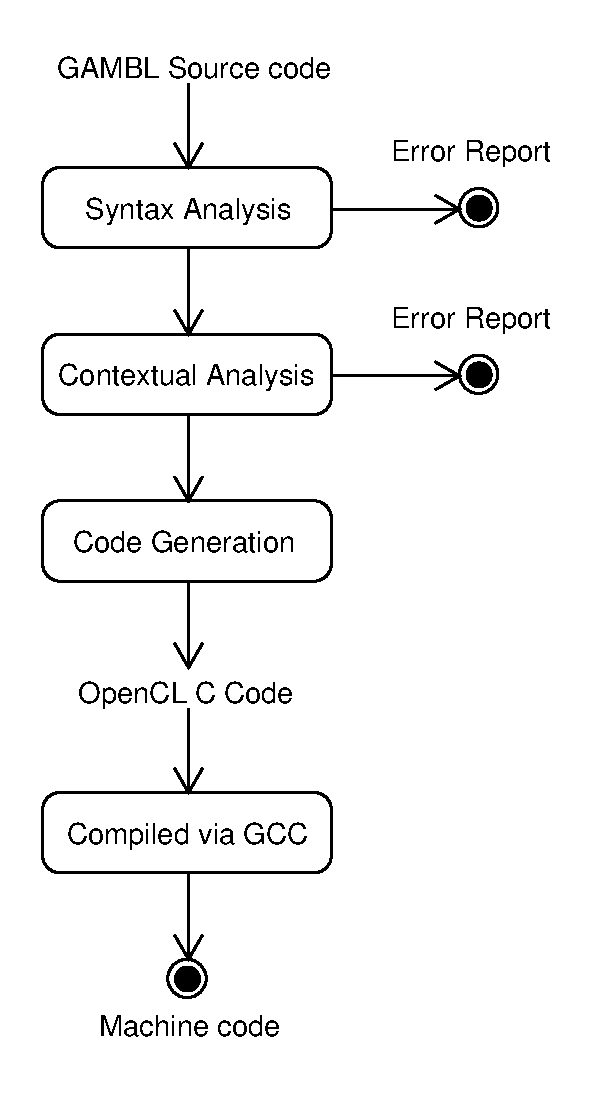
\includegraphics[width=0.5\textwidth]{figures/ClassDiagrams/CompilerDiagram.pdf}
\caption{State diagram showing the phases of the compiler when it takes \gls{gamble} source code and compiles it into machine code.}\label{fig:phases}
\end{figure}

\begin{figure}[t]
	\begin{sideways}
	%\fbox{
		\begin{minipage}{22.5cm}
			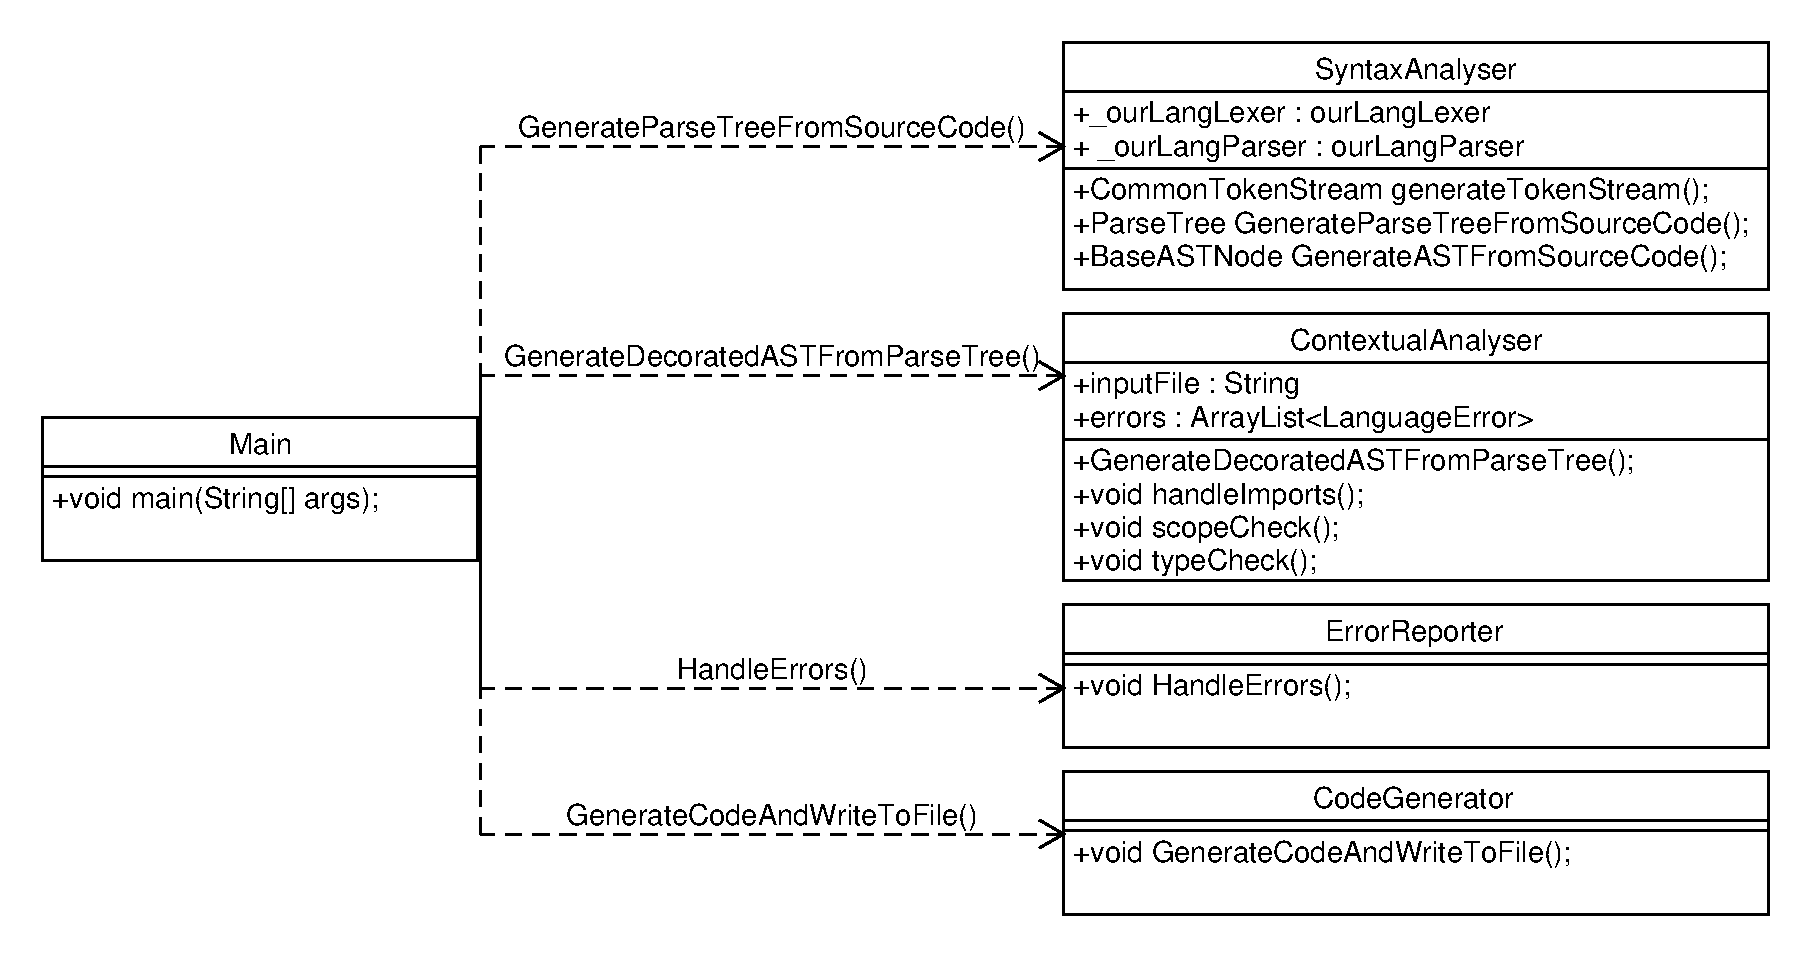
\includegraphics[height=0.42\textheight]{figures/ClassDiagrams/DiagramOfCallsFromMain.pdf}
		\end{minipage}
	%	}
	\end{sideways}
	\centering
	\caption{Diagram showing the structure of the compiler by showing the \texttt{main()} method's method calls. Arguments are omitted for simplicity}\label{fig:compilerOverview}
\end{figure}


%\begin{figure}[ht!]
%	\centering
%	\begin{tikzpicture}[node distance = 2.5cm]
%		\node (invi1) 		[invi,draw=none] {GAMBLE Source code};
%		\node (syntax) 		[blockz, below=0.6cm of invi1] {Syntax Analysis};
%		\node (contextual) 	[blockz, below of=syntax] {Contextual Analysis};
%		\node (codegen) 	[blockz, below of=contextual] {Code Generation};
%		\node (opencl) 		[invi,draw=none, below=0.6cm of codegen] {OpenCL C code};
%
%		\node (error1) 		[cloud, right=1cm of syntax] {Error reports};
%		\node (error2) 		[cloud, right=1cm of contextual] {Error reports};
%
%		\node (invi2) 		[invi,draw=none, below=0.4cm of syntax] {};
%		\node (ast) 		[invi,draw=none, right=-0.2cm of invi2] {Abstract Syntax Tree};
%
%		\node (invi3) 		[invi,draw=none, below=0.4cm of contextual] {};
%		\node (dast) 		[invi,draw=none, right=-0.5	cm of invi3] {Abstract Syntax Tree \& Symbol Table};
%
%		\draw [arrow] (invi1) -- (syntax);
%		\draw [arrow] (syntax) -- (contextual);
%		\draw [arrow] (contextual) -- (codegen);
%		\draw [arrow] (codegen) -- (opencl);
%		
%		\draw [arrow] (syntax) -- (error1);
%		\draw [arrow] (contextual) -- (error2);
%	\end{tikzpicture}
%	\caption{The phases of the compiler.}\label{fig:phases}
%\end{figure}
\clearpage

\label{SourceCodeAsTrees}
\todo{Write about Sourcecode as Trees, and why we do that.}

\chapter{Syntax Analysis}\label{sec:syntaxAnalysis}
Syntax analysis is the first phase in compiling a language.
In this phase it is checked whether the input adheres to the rules of the language.
These rules are defined in a languages' \acrshort{cfg}.
The \acrshort{cfg} of \gls{gamble} is further described in \myref{sec:cfg}.
This analysis can be split up into further sub phases, lexical analysis and parsing, these are described in this chapter.

\vspace{10pt}
\begin{figure}[h]
    \centering
    \begin{tikzpicture}[node distance = 3cm, auto]
        \node (start) [lille] {Source code};
        \node (scanner) [lille, right=0.7cm of start] {Scanner};
        \node (parser) [lille, right=0.7cm of scanner] {Parser};
        \node (pt) [lille, right=0.7cm of parser] {Parse--Tree};
        \node (ast) [lille, right=0.7cm of pt] {Abstract Syntax Tree};
        \node (error) [cloud, above=1cm of parser] {Error report};

        \draw [arrow] (start) -- (scanner);
        \draw [arrow] (scanner) -- (parser);
        \draw [arrow] (parser) -- (pt);
        \draw [arrow] (pt) -- (ast);
        \draw [arrow,dashed] (parser) -- (error);

    \end{tikzpicture}
    \caption{Diagram showing the modules of the syntax analysis. } 
    \label{fig:flowSyntax}
\end{figure}
\vspace{-20pt}

\section{Design}
%Design
\subsection{Scanner}
The first stage of syntax analysis is the scanner, also called the lexer which handles the lexical analysis.
The primary function of a scanner is to transform a sequence of characters into a sequence of tokens.
The scanner makes sure that the source code adheres to the grammar rules provided by the CFG.
An example of this, would be that you could use the notation .1 or 0.1 for a decimal number, both being turned into valid tokens by the scanner.
The scanner provided by ANTLR groups related tokens into token types such as INT, ID and FLOAT.
In ANTLR a token contains at least two pieces of information, the token type and the matched text for the token.

Some examples of our lexical rules for \gls{gamble} can be seen on \myref{lst:token}.
The definition of an integer number on line 3 states that an integer is either a zero or an optional negative sign followed by a single digit from one to nine followed by zero or more numbers from zero to nine.
It is necessary to clearly define tokens for the lexer to read in order to read source code correctly. \citep{Crafting_book}

\begin{lstlisting}[caption=Example of our lexer rules for ANTLR4,frame=tlrb,label={lst:token}]
// Integers
INT: 'int' | 'int16' | 'int32' | 'int64' ; // Integers
INTNUM: '0' | SIGN? [1-9][0-9]* ;

// Matrices and vectors
MATRIX: 'matrix' ;
ROWVECTOR: 'rowvector' | 'rvec' ;
COLVECTOR: 'colvector' | 'cvec' ;  

// Whitespace and comments
WS: [ \t ]+ -> skip;
NL: [ \r \n | \n ] -> skip;

COMMENT
    :   '/*' .*? '*/' -> skip
    ;

LINE_COMMENT
    :   '//' ~[\r\n]* -> skip
    ;
\end{lstlisting}
\subsection*{Parser}\label{subsec:parser}
The parser is based on the \acrfull{cfg} of \gls{gamble} written in \acrfull{ebnf}, whose alphabet consists of tokens produced by the scannar.
The parser reads tokens and groups them into phrases according to the \acrshort{cfg}.
The parser verifies that the syntax is correct and upholds to the \acrshort{cfg}, and if a syntax error is found it provides a corresponding error message. \citep{Crafting_book}
By using a parser generator like \acrshort{antlr} or SableCC, handling of syntactic errors and repairs can be done automatically.
A parser can also be written manually but doing so can result in syntactic errors that is hard to locate or solve.
Writing a parser by hand can also take a lot of time, and it can be difficult to go back and change or add new productions to the syntax, which is something the project group will want to do due to the iterative development.
There are many parser generators which can be used like: SableCC, JavaCC, JFlex and many others, but we have chosen to use \acrshort{antlr}.
\acrshort{antlr} has been chosen due to their special use of the ALL(*) grammar, which poses many opportunities for the grammar, and also makes the \acrshort{cfg} easier to write.
\acrshort{antlr} generates a parser which produces a parse tree that contains information about how the parser have grouped the tokens into more abstract language definitions, such as expressions and statements.

There are different kind of parsers, most common are bottom-up and top-down parsers.
\acrshort{antlr} makes a top-down parser, more specific a recursive descent parser.
A recursive descent parser is a subtype of top-down parser build from a set of mutually recursive procedures where each such procedure implements one of the productions of the grammar.
The structure of the resulting program closely mirrors the grammar it recognizes. \citep{Recursive_programming}
Recursive-descent parsers are a collection of recursive methods, one per rule of the \acrshort{cfg}.
Such a method for an assignment rule may look as shown in \myref{lst:rdpmethod}, where the rule is \texttt{assignment : ID = expr ;}.
So the method expects an ID to be the first token from the tokenstream, then an assignment operator followed by an expression and a semicolon.
Here the expression is a rule itself, and is therefore called on the expected expression.
An error should be returned if anything is not what was expected.
\begin{lstlisting}[caption=Example a recursive descent parser method,frame=tlrb,label={lst:rdpmethod}]
// assign : ID ``='' expr ``;'' ;
void assign() { // method generated from rule assign
match(ID); // compare ID to current input symbol then consume
match('=');
expr(); // match an expression by calling expr()
match(';');
}
\end{lstlisting}

%The second stage of the parser is the actual parser.
%The parser is fed a stream of tokens to recognise a sentence structure and in turn outputs the structure to a parse tree.
%The parse tree records how the parser recognises the structure of the input and its components.
%The parse tree that \acrshort{antlr} provides contains information about how the parser have grouped the tokens into more abstract languange definitions such as expressions and statements.
%Where previous versions of \acrshort{antlr} have also implemented the AST, it is not contained in \acrshort{antlr} V4 instead the parse tree provided by \acrshort{antlr} have been used to generate an AST this is discussed in \myref{sec:AST}.
%This tree is a trimmed version of the parse tree, where the less informative data have been removed, this makes it easier to read, and thus easier to use throughout development of the rest of the compiler.

%2nd stage is the actual parser, feeds of tokens to recognize sentence structure
%Parse tree records how the parser recognized structure of input and its component phrases
%Trees provide an easy to walk data structure that will be helpful for the rest of the compiler
%2.2 Implementing Parser - Recursive descent
%Recursive-descent parsers are really just a collection of recursive methods, one per rule.
%Such a rule may look similar to this
%// assign : ID ``='' expr ``;'' ;
%void assign() { // method generated from rule assign
%match(ID); // compare ID to current input symbol then consume
%match('=');
%expr(); // match an expression by calling expr()
%match(';');
%}
%Descent refers to the fact we start from the root and go down to the leaves(tokens)
%Reursive descent is just one form of top-down parsers.					NOTE topdown/bottom up parsing
%The call graph traaced out by invoking methods, mirrors the interior parse tree nodes
%To Build a parse tree manually one would insert ``add new subroot note' operations at the start of each rule, and a ``add new leaf node'' operation to match()
%The assign method checks if all necessary tokens are present and in the right order. When the parser enters assign it doesnt have to choose between more than one alternative. An alternative is one of the choices on the right side of a rule def. A parsing method for such rule would be a switch which looks for what token is present.
% This is called a parising decision or prediction by examining next token
%This is where lookahead comes into play , the lookahead token is the next input token, this can be any token the parser "sniffs" before consuming
%This is one of the places where \acrshort{antlr} is an especially handy tool to use, because \acrshort{antlr} allows for more lookahead than other parser generators.
%Most parsers use a lookahead of one which LL(1) or LR(1), \acrshort{antlr} tones the lookahead up and down depending on what token stream it is trying to decode, as such the \acrshort{antlr} has a lookahead of LL(*)
%\acrshort{antlr} Solves simple ambiguity simply by using the first mentioned rule.
%AST only useful, Parse all artifacts(space, brackets and so on)


\subsection*{Abstract Syntax Tree}
\todo{to be written}
\subsubsection*{Traversal of Trees}
In the previous section an \acrshort{ast} which contains information from the source code was presented; to get the information from the trees, a tree traversal is needed.
For this task different approaches can be taken, one way is to implement a design pattern called the visitor pattern.
Alternatively one can implement the composite pattern or choose to implement no pattern at all, but simply create a case analysis for each object.
The use of a design pattern is not a requirement for the creation of a compiler.

Design patterns provide a general reusable solution for a software problem, each pattern providing its own benefits.
Using a pattern is not just copy and pasting other's code, but it simply states how to solve the problem at hand using different software structures.\todo{Copy pasting code? Hænger det sammen med design patterns? - Corlin}
In OOP, patterns are often described from a UML diagrams, showing the class and interface structure, and which methods these classes must implement. 

The two aforementioned patterns are classified under two different branches of patterns.
The composite pattern is a structural pattern where the visitor pattern is a behavioural one.
A structural pattern provides a way of defining the relations between objects, the composite pattern is used to create a hierarchical recursive tree structure of related objects that may be accessed in a standardised manner.
A behavioural pattern is instead used to define how the objects communicate, the visitor pattern is used to separate a set of structured classes from any functionality that should be performed upon them.\citep{GOF}
For the compiler the visitor pattern have been implemented for the traversal of trees as such the pattern is described further in the following section. 

\subsubsection*{Visitor Pattern}\label{subs:visit}
The visitor pattern is not only used to traverse the parse tree provided by ANTLR, but also the \acrshort{ast} created in the compiler.
The visitor pattern is implemented throughout the compiler, to create the \acrshort{ast} from the parse tree and for traversing the \acrshort{ast}.
As such the visitor pattern defines the structure of the compiler, and thus understanding the benefit from using the pattern is important.
The visitor pattern is described by the Gang of Four, authors of ``Design Patterns: Elements of Reusable Object-Oriented Software'' as:
``a design pattern that separates a set of structured data from the functionality that may be performed upon it.''. \citep{GOF}

In the tree walk for the parse tree, the visitor should convert the parse tree into a \acrshort{ast}.
This entails that each different node in the parse tree must be visited to find the information needed to create the \acrshort{ast}.

Through use of the visitor pattern the functionality is separated from the classes they are performed upon. 
Instead the functionality is on a visitor class implementing the visitor interface, which means different visitors can be made, which all do different computations while traversing the tree.\todo{måske tasks i stedet for computations. MP}
Each class in the tree have an \texttt{accept()} method that allows them to call the visitor in question with itself as an argument.
This allows the ability of adding new operations without changing the original data structure, and also without changing other visitors.
This also serves well when using a iterative development method.
Another benefit is that a single visitor object is used to visit all the classes in the tree.
This visitor can therefore maintain a state between calls to individual data objects, which can be used to save information in an outer scope from the different visit calls.
\myref{image:visitor} shows an UML diagram of the visitor pattern.
This diagram is from a C\# representation, and while the idea is the same the exact implementation is not identical to the one used in the compiler for \gls{gamble}.
Take note of the classes ``ConcreteElement'' and ``ConcreteVisitor''.
The ``ConcreteElement'' represents the different kinds of nodes in a given tree.
The ``ConcreteVisitor'' represents the different kind of visitors implemented.
A visitor will make sure that the children of the node is traversed in the correct way, and will at the same time also do other computations, e.g. pretty printing or checking the source code for errors.\todo{Skal vi komme med andre eksempler her ? Såsom, type checking or code generating?}
A visitor must implement a method to visit every single ``ConcreteElement'' which exist in the tree.
As can be seen on \myref{image:visitor} ``ConcreteVisitorA'' and ``ConcreteVisitorB'', both implement a visit method for the ``ConcreteElements'' A and B.
In the next section, the implementation of creating the \acrshort{ast} from the parse tree using the visitor pattern will be presented.

\begin{figure}[!ht]
\centering
 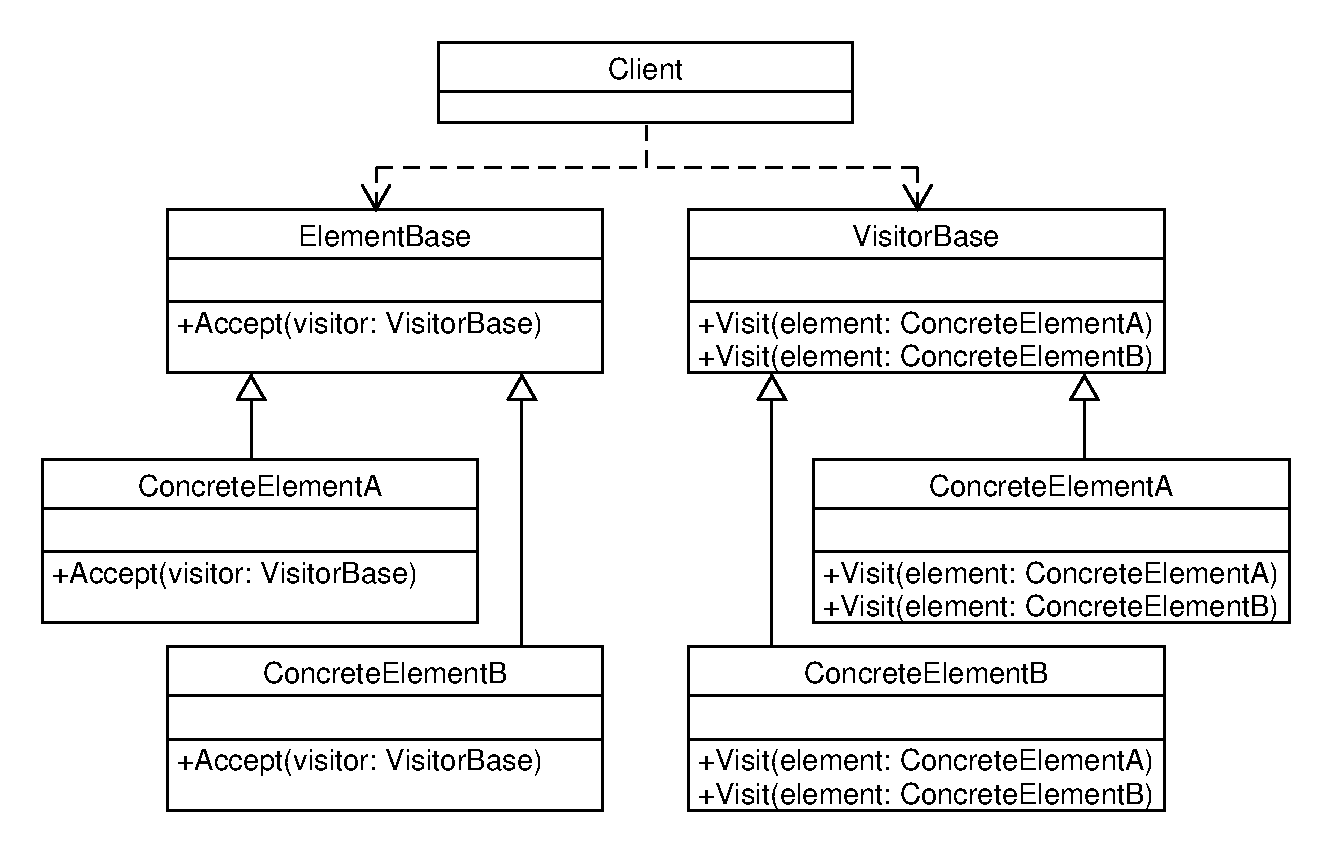
\includegraphics[width=1\textwidth]{figures/ClassDiagrams/VisitorPattern.pdf} % trim=4.85cm 15cm 0.85cm 1cm
\caption{An UML diagram for the implementation of the visitor pattern.}\label{image:visitor}
\vspace{-15pt}
\end{figure}
\todo[inline]{har vi selv lavet figuren? MP - Ja den har jeg lavet :) men der skal nok en kilde på så man kan se hvor vi har det fra, Marc found it. - Søren}

\subsection{Creating the \acrshort{ast}}\label{CreatingAst}

The goal for the \acrshort{ast} is to decrease the information in the tree.
The hidden information is then contained in fields created for the respective classes.\todo{Kan ikke finde ud af om det er lidt for groft at sige hidden information? - Søren}
Rather than having the information as fields one could also choose to have this information as children of the nodes.
This would mean that to find the information one would have to run through the children of the nodes without knowing what children it has.
The method chosen for this compiler has the information kept on the fields of a node rather than as children.
The advantage being that the information is kept together without clustering the tree and increasing the readability of the compiler.
All the nodes of the \acrshort{ast} have been designed with this in mind.
For example on figure \myref{image:ASTDecl} a class structure can be seen, which consists of all the classes needed to express a declaration from the \acrshort{cfg} on the tree.
A declaration could be \texttt{int a = 5;}.

\begin{figure}[!ht]
\centering
 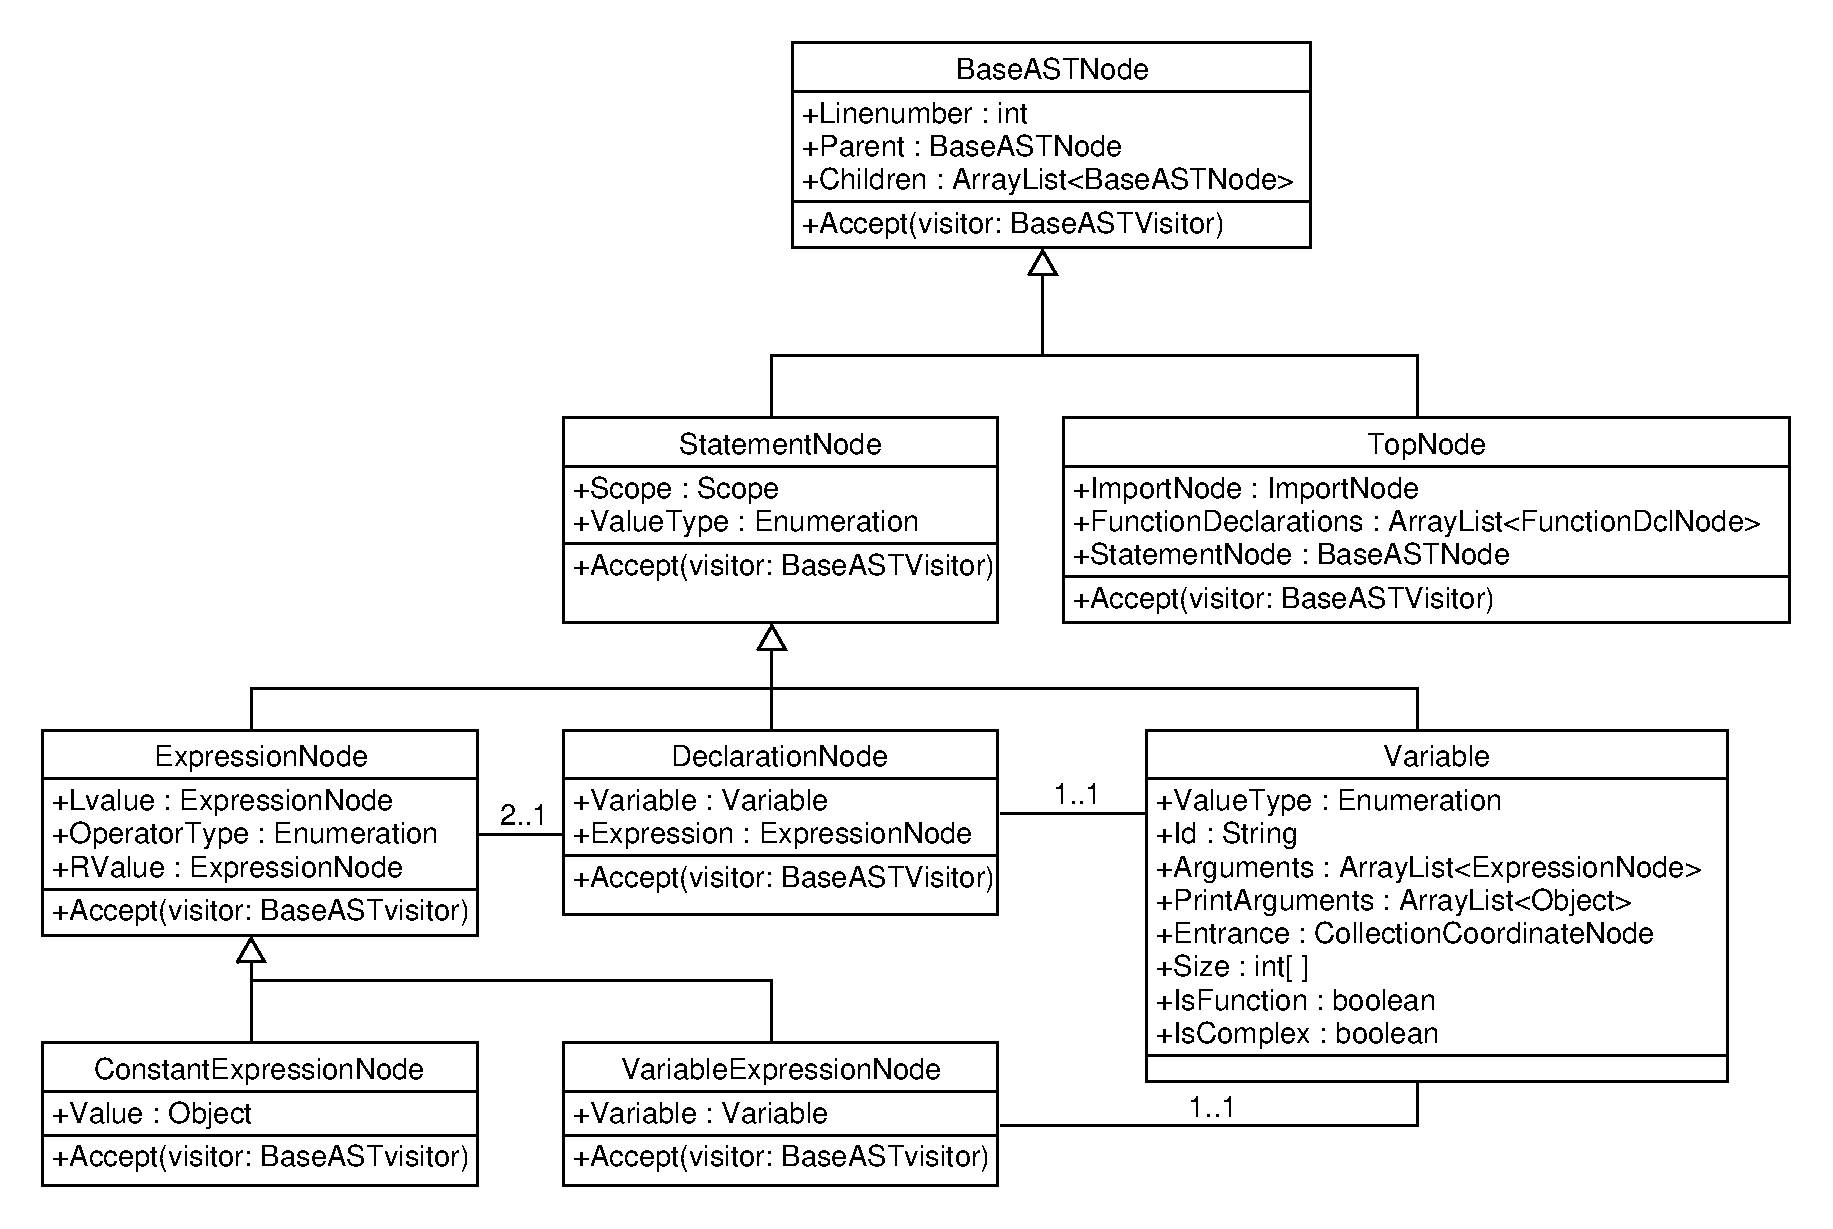
\includegraphics[width=1\textwidth]{figures/ClassDiagrams/ASTDeclarationNodeMoreInfo.pdf} % trim=4.85cm 15cm 0.85cm 1cm
\caption{A UML class diagram of the classes used for a DeclarationNode on the \acrshort{ast}.}\label{image:ASTDecl}
\vspace{-15pt}
\end{figure}

The \texttt{Variable} class contains a lot of different information which is used depending on which class a given instance of \texttt{Variable} is connected to.
If \texttt{Variable} is connected to a \texttt{VariableExpressionNode}, the only fields used on the variable class is ValueType and Id, while the booleans IsFunction and IsComplex are set to false.
In the example \texttt{int a = 5;} the tree structure looks like the AST on \myref{image:AST}.
When the right hand side of an assignment or declaration is a function, an example being \texttt{int a = foo(5);} the fields used on \texttt{Variable} differs from the previous example and instead becomes Id, ValueType, arguments, and the boolean IsFunction is now set to true.
The print argument field is used when a function call to \texttt{print()} is made. 
Entrance, Size and IsComplex are used when dealing with the complex data types, vectors and matrices.
\texttt{TopNode} sets the structure of a \gls{gamble} program as described in \myref{subsec:Struc}.
The full class diagram can be seen in \myref{ASTNodes}.

The classes have made it more intuitive to perform a traversal of the tree based upon the names of the fields on the classes.
E.g. the \texttt{ForLoopNode} has fields named \texttt{Body}, \texttt{Initialize}, \texttt{Update}, and \texttt{Conditional}, these names have meaning instead of just being children on the node which will increases the readability of the compiler.

The syntax analysis phase returns the \acrshort{ast} so it can be used in the next phase, the contextual analysis. 
The design of the phase and the call from main can be seen on \myref{fig:syntaxphase}.\todo{call from main kunne thomas ikke lide. MP - Tror det var fordi han ikke havde set figuren i compiler overview som viser alle kaldene fra main, og dermed var han forvirret over det ? Men ved det self ikke, synes bare ikke det gør noget når man også har set den figur. - Søren}
As can be seen the \texttt{GenerateASTVisitor} makes use of the classes shown in \myref{ASTNodes}.

\begin{figure}[ht]
  \centering
    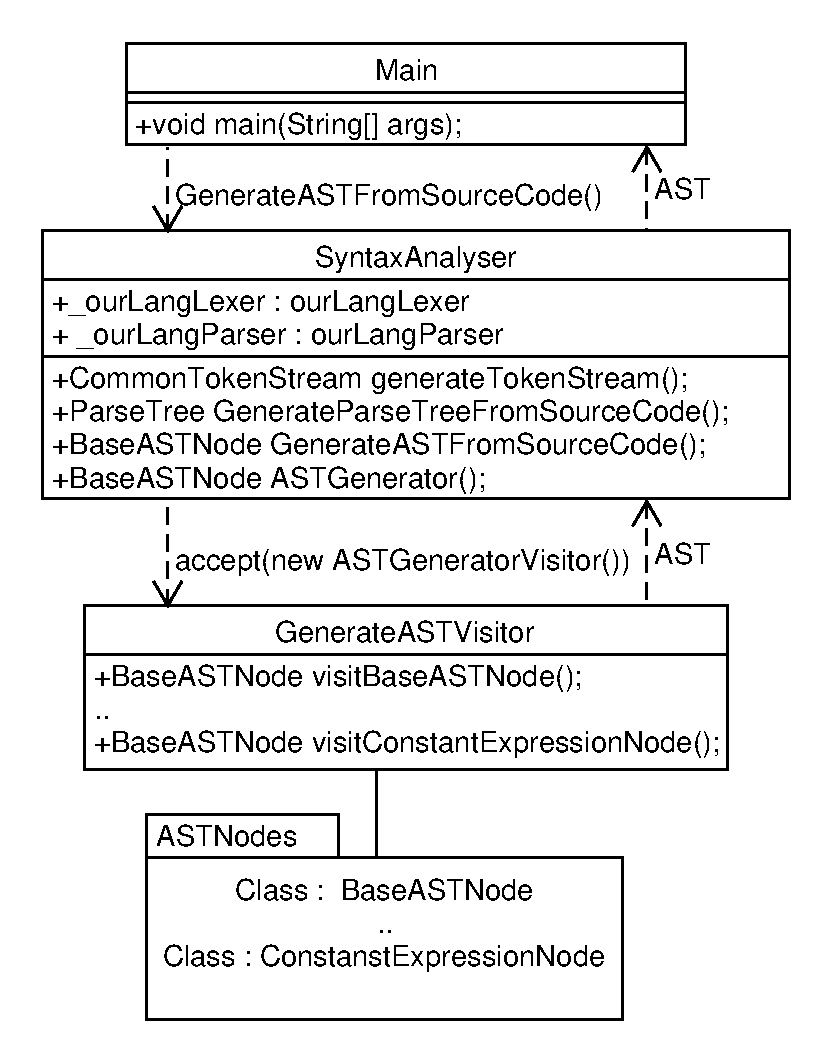
\includegraphics[width=0.48\textwidth]{figures/ClassDiagrams/SyntaxAnalyser.pdf}
  \caption{The function calls and returns in the Syntax Analysis phase.}
  \label{fig:syntaxphase}\todo{Skal vi vise at generateParseTreeFromSourceCode kaldes af ASTFromSourceCode eller noget ? - Søren}
\end{figure}

%Implementation
\section{Implementation}\label{sec:ANTLR}
The syntax analysis is implemented through the tool \acrfull{antlr}, this tool provides some advantages over other available tools.
\acrshort{antlr} is based upon a parser technique called LL(*).
LL(*) uses an algorithm to have a varying lookahead when needed.
The LL(*) parsers, which is a parser that upholds an LL(*) grammar, does not allow a bigger class of \acrshort{cfg}s than other parsers like LL(k), but can change the number of tokens needed as lookahead dynamically. 
In the most recent version of \acrshort{antlr} as time of this publication, \acrshort{antlr}4, the underlying algorithm have been extended to a parser technique called Adaptive LL(*) (ALL(*)).
An important feature of ALL(*) is it moves grammar analysis to parse time and thereby lets the algorithm accept any non-left-recursive productions.
On top of that \acrshort{antlr} allows simple left recursions by rewriting them before parse time.

The \acrshort{antlr} approach accepts a broader class of grammars than most other parsing methods, one way this is done is to rule out ambiguity by using a rule of precedence.
If a grammar is ambiguous the ALL(*) approach will take the first available rule in the \acrshort{cfg} and apply it.
This allows for more opportunities in the \acrshort{cfg} and while most grammars could be rewritten to be unambiguous without applying the precedence rule.
The idea with the ALL(*) algorithm is that the grammar is analysed at parse-time, and requires no static analysis of the grammar. 
This means that the undecidability of static LL(*) grammar analysis is avoided and instead it is possible to make correct parsers for any non-left-recursive \acrshort{cfg}.
This allows \acrshort{antlr} access to input sequences while reading through the grammar, meaning not all possible inputs must be considered.
Due to this dynamic analysis \acrshort{antlr}4 is able to handle some ambiguous constructs and reduce-reduce conflicts.
As mentioned this allows \acrshort{antlr} to take care of left-recursion if such is present in the grammar by rewriting it, as such would be the case in \myref{lst:amb}.

\begin{lstlisting}[caption=An ambiguous rule for expr, which ANTLR handles by applying the first rule of the production if possible,frame=tlrb,label={lst:amb}]
expr : expr '*' expr 	#MulExpression // match expressions with * operator
     | expr '+' expr 	#AddExpression// match expressions with + operator
     | INT 		// matches simple integer
     ;
\end{lstlisting}
\myref{lst:amb} implements \acrshort{antlr}s way of representing operator precedence by simply obeying the first alternative in the rule set, as such the multiplication operator (``*'') will have the higher precedence.
The ALL(*) algorithm also means that one can completely disregard lookahead and it will still be able to parse, although one should keep in mind that having more lookahead than necessary will slow down the process of parsing.
The scanner provided by \acrshort{antlr} groups related tokens into token types such as INT, ID and FLOAT.
In \acrshort{antlr} a token contains at least two pieces of information, the token type and the matched text for the token.
\acrshort{antlr} also implements rule element labels in its \acrfull{cfg} which means one can apply label rules to a construct in a grammar, this allows for conditional steps in the grammar based on the source code being parsed.
The labels on \myref{lst:amb} are \texttt{\#MulExpression} and \texttt{\#AddExpression}.
Furthermore \acrshort{antlr} can set up an interface and base implementation of the visitor pattern for the parse tree on a given grammar by running \acrshort{antlr} with the \texttt{--visitor} flag. \citep{ALLSTAR, LLSTAR, antlr4_Book}

\subsubsection*{Implementation of Creating the \acrshort{ast}}

The class \texttt{VisitorAST} creates the \acrshort{ast} from the parse tree, it traverses the tree using the visitor pattern and on every node sets a field of a class in the \acrshort{ast}. 
Afterwards the node is placed on the tree as a leaf or a field on the node which made the \texttt{visit()} call.

One of these visit methods can be seen on \myref{lst:VisitorASTCode}.

\begin{lstlisting}[caption=The visit method for WhileLoopNode,frame=tlrb,label={lst:VisitorASTCode}]
public BaseASTNode visitWhileLoop(ourLangParser.WhileLoopContext ctx) {
    WhileLoopNode whileLoopNode = new WhileLoopNode(parentStack.peek());
    whileLoopNode.setCondNode(
    	(ConditionalExpressionNode)visit(ctx.conditionalExpression()));
    parentStack.push(whileLoopNode);
    visitChildren(ctx.whileBlock);
    parentStack.pop();
    whileLoopNode.setLineNumber(ctx.start.getLine());
    return whileLoopNode;
}
\end{lstlisting}
A stack called the parentstack is used to keep track of the caller to \texttt{visit()}, in order to keep track of the parents and the children of the tree.
On lines three and four on \myref{lst:VisitorASTCode} a call to visit the \texttt{conditionalexpression} of the whileloop is made, which returns an instance of the class \texttt{ConditionalExpressionNode}.
Afterwards, to set the body of the \texttt{WhileLoopNode}, all the children of the nodes are visited, but first the \texttt{WhileLoopNode} is pushed to the parentstack.
This makes it possible to check which node is the parent of the children being created during the calls to visit.
\acrshort{antlr} uses the implementation where each node has a number of children, and therefore the \texttt{WhileLoopContext} has its children visited rather than specific fields.
While implementing the Visitor pattern for the \acrshort{ast} an interface was made, which contains a visit method for every single class of the \acrshort{ast}.
A baseclass which implements this interface which implements a visit method for all the nodes of the \acrshort{ast} such that the correct fields of the nodes are visited in the intended order.
This means that any visitor class only has to override the visit methods which are of interest for the specific visitor and the ones not overridden will use the baseclass' implementation which simply visits its fields.
An UML diagram for the implementations of the visitor pattern in the compiler and can be seen on \myref{image:Visitors}.
The figure shows how every visitor class inherits from the \texttt{BaseASTVisitor} class.\todo{Overvejer lidt om denne figur skal væk da det jo er design og egentlig bare viser det som figuren i design viser? - Søren}
Now that the Syntax analysis phase is done it is time for the \acrshort{ast} to be send to the contextual analysis phase which the next chapter will cover.

\begin{figure}[!ht]
\centering
 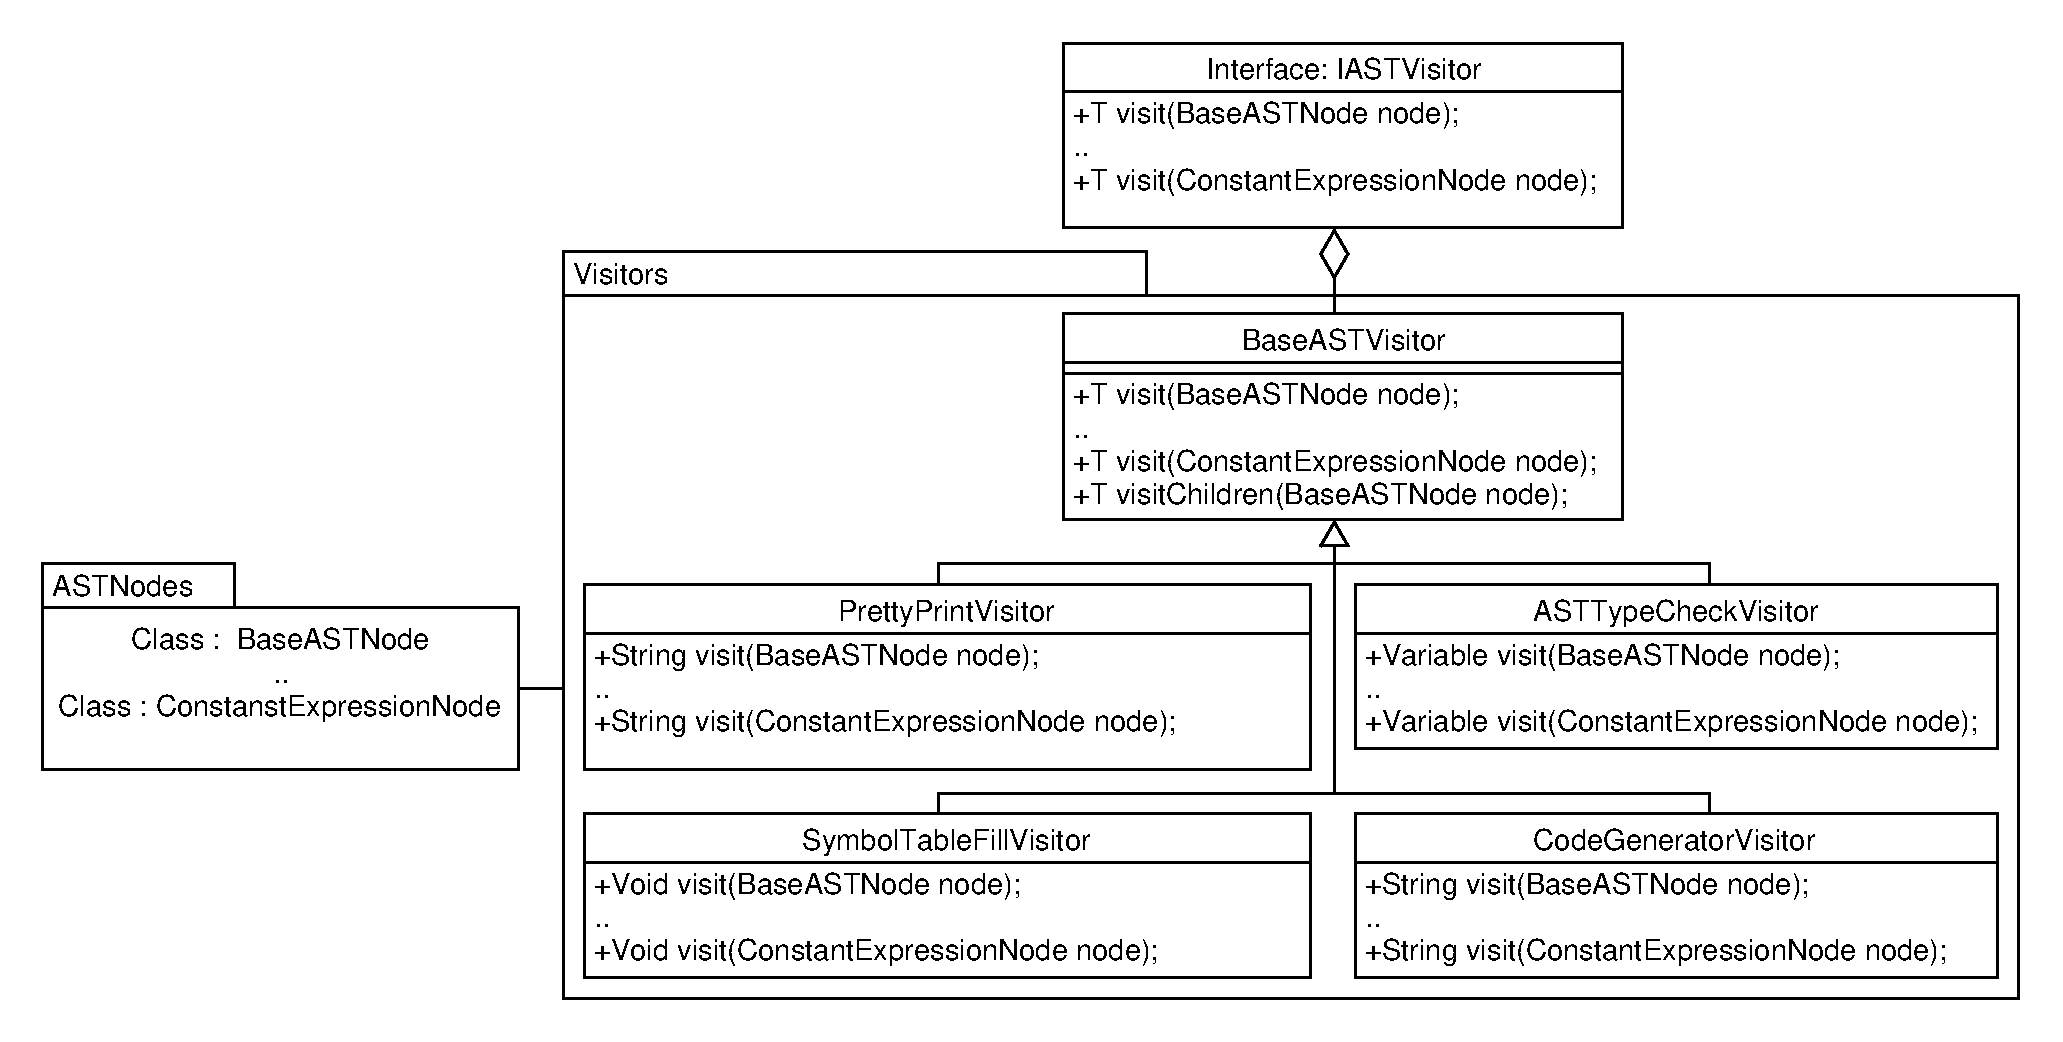
\includegraphics[width=1\textwidth]{figures/ClassDiagrams/Visitors.pdf} % trim=4.85cm 15cm 0.85cm 1cm
\caption{An UML diagram of the visitor patterns implementation in the compiler for traversing the \acrshort{ast}.}\label{image:Visitors}
\vspace{-15pt}
\end{figure} 

%Subphases
\chapter{Contextual Analysis}
Once the source code has passed through the syntax analysis, and thereby is validated in regard to the \acrshort{cfg}, it must be checked for contextual errors.
In the contextual analysis phase semantic errors are the ones being checked for, this includes type errors such as type mismatch, e.g. adding a boolean to a float, which may well be using the correct grammar, but is not a valid arithmetic expression.
In the contextual analysis there is also checked in which scopes the different variables is available and if there is errors of this type.
The design and implementation of the contextual analysis as well as how such errors are handled are described in this chapter.

The contextual analysis phase has sub-phases for scope- and type-checking and error handling.
An illustration of the design for this can be seen on \myref{fig:flowContextual}

\begin{figure}[ht]
  \centering
    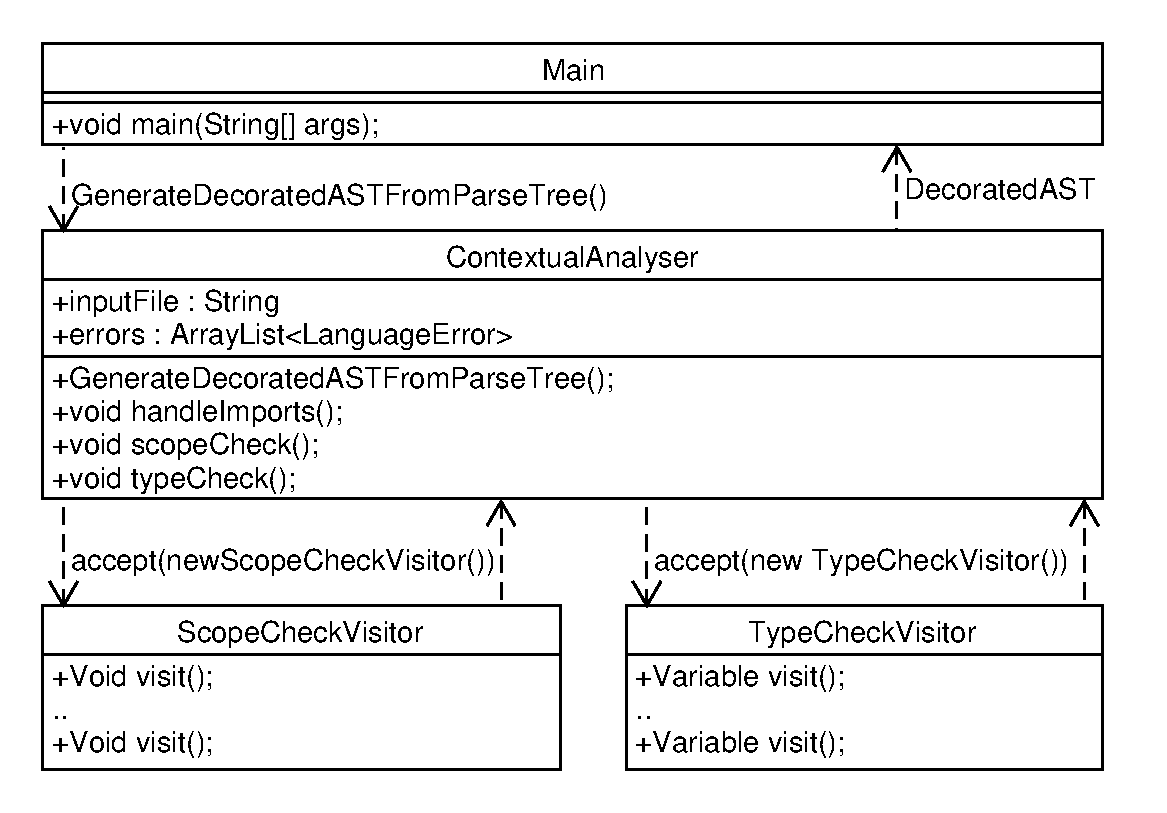
\includegraphics[width=0.48\textwidth]{figures/ClassDiagrams/ContextualAnalyser.pdf}
  \caption{The function calls and returns in the Contextual Analysis phase. \todo[inline]{Delete this, replaced by flowchart? -- Troels}}
  \label{fig:Contextual}
\end{figure}

\vspace{10pt}
\begin{figure}[h]
    \centering
    \begin{tikzpicture}[node distance = 3cm, auto]
        \node (invi1) [invi, draw=none] {};
        \node (snyanal) [lille, below right=-2cm and -1.6cm of invi1, minimum width=15.5cm, minimum height=5cm, fill=blue!10, label={[xshift=-5.4cm, yshift=-1cm]Contextual Analysis}] {};
        \node (ast) [lille, below right=-0.35cm and -1cm of invi1] {Abstract Syntax Tree};
        \node (symboltable) [lille, minimum width=6.75cm, minimum height=2.4cm, right=2.8cm of invi1, fill=blue!20, label={[xshift=0cm, yshift=-1cm]Symbol Table}] {};
        \node (scope) [lille, right=1.1cm of ast] {Scopechecker};
        \node (type) [lille, right=0.7cm of scope] {Typechecker};
        \node (dast) [lille, right=1.1cm of type, align=left] {Decorated\\ Abstact Syntax Tree};
        \node (codegen) [lille, right=1.1cm of dast, align=left] {Code \\Generation};

        \node (error) [invi, draw=none, minimum width=2cm, below=1cm of symboltable, label={[xshift=40pt, yshift=-17pt]Error report}] {};

        %\node (error) [draw=none, above=22pt of parser, label={[xshift=0cm, yshift=6 pt]Error report}] {};

        \draw[black,fill=black, above=1cm of parser] (6.35,-2.5) circle (1ex);
        \draw[black, above=1cm of parser] (6.35,-2.5) circle (1.3ex); 

        \draw [arrow] (ast) -- (scope);
        \draw [arrow] (scope) -- (type);
        \draw [arrow] (type) -- (dast);
        \draw [arrow] (dast) -- (codegen);

        \draw [arrow,dashed] (scope) -- (error);
        \draw [arrow,dashed] (type) -- (error);
        \draw [arrow,dashed] (symboltable) -- (error);

    \end{tikzpicture}
    \caption{State diagram showing the modules of the contextual analysis. } 
    \label{fig:flowContextual}
\end{figure}
\vspace{-20pt}

%\section{Contextual Analysis}
\info[inline]{meta for this, phases are done in their own subsection files}
\section{Symbol Table}
In a compiler it is useful to store information about the identifiers, variables and functions in a data structure. 
This information can be useful for scope checking and type checking.

There are two common ways of implementing a Symbol Table; either you have one table which contains every identifier or you have a Symbol table for each scope. 
If constrained by memory, having a single symbol table can be beneficial, however having multiple symbol tables can simplify the code at a memory cost. 

In \gls{gamble} there exists scopes, and for each of these scopes there is a corresponding symbol table. 
Scopes inherit from each other so a scope can enclose another. 
The outermost scope, the global scope, is where functions are declared; every scope is either directly enclosed by this scope or recursively.
This means that every function can be called from anywhere within the source code - including within its' own function declarations; allowing for recursive functions. 
  

\info[inline]{Flyttes til implementationsafsnit $\downarrow$ }
In \gls{gamble} the class \texttt{SymbolTable} represents the symbol table.
The core constituent of this class is the ArrayList of the Scope class, called allScopes, meaning that every scope is stored in this ArrayList.
Every scope contains Map of Symbols and strings as keys, and information about the scope such what scope it is enclosed by. 
The key represents the name of the symbol, and must be unique to the scope and not found in an enclosing scope, as this could cause an ambiguity to arise. 
A symbol is either a variable or a function, in the class Symbol its data type, name and scope is stored. 


\section{Scope Checking}
As a part of the contextual analysis the compiler must ensure that every reference is valid in their given scope.
The validity of such reference is specific to the rules of the language, this section describes how the compiler upholds the rules listed in \myref{subsec:Scope}.
\subsection*{Design}
In \myref{subsec:Scope} the scope of identifiers, variables and functions, are defined for \gls{gamble}.
A variable is in scope from its declaration until the end of the block it is declared in.
An inner scope inherits the identifiers declared in the outer scopes. 

In the contextual analysis part of the compiler it is important to verify that each variable and function used are in scope, and it should produce a useful error message.
The error message should indicate which identifier is not in scope, and on what line this identifier is used wrongly.

To check this all references to identifiers must be checked to see if they match an identifier in the symbol table of the current scope, and recursively the scope which encloses it. 
Furthermore it is important that any usage of an identifier only exists after its declaration.
In the compiler for this project, the symbol table is filled while the compiler is also performing the scope checking.
This is because it reduces the amount of traversals through the tree, and scope checking and filling the symbol table is also similair in concept, e.g. a declaration creates an entry in the symbol table, while expressions simply make lookups in this table.

The scope checker produces two errors: redeclaration errors and undeclared errors.
A redeclaration error is produced when an attempt to declare a variable while it is already declarared in scope is made.
An undeclared error is produced when an attempt to use a variable which is not declared in the current scope or any enclosing scopes is made. 
Examples are shown in \myref{lst:scopeErrors}.

\begin{lstlisting}[caption=Examples of scope errors in \gls{gamble}, numbers=none,frame=tlrb,label={lst:scopeErrors}]
/* [...] */
int a = 1;
float a = 2.2;   /* Redeclaration error */
int a = 2;       /* Redeclaration error */ 

b = 2;           /* Undeclared error */   
int b = 0;
b = foo();       /* Redeclaration error and undeclared error */ 
/* [...] */
\end{lstlisting}

\subsection*{Implementation}
In the \gls{gamble} compiler, the class \texttt{SymbolTable} represents a collection of scopes.
The core constituent of this class is the ArrayList of the \texttt{Scope} class, called \texttt{allScopes}, meaning that every scope is stored in this ArrayList.
Every scope contains a hashed map with \texttt{Symbol}s as values and strings as keys.
Furthermore all scopes contain information about the particular scope such as enclosing scope and a unique id. 
The key in the hashed maps represents the name of the symbol, and must be unique to the scope and not found in an enclosing scope, as this could cause an ambiguity to arise.
This ambiguity is not allowed in \gls{gamble} and therefore generates a redeclaration error.
To determine wether or not a declaration is a redeclaration, the compiler looks up the name of the variable in the \texttt{symbolMap} of the current scope.
If no entry is found, the search continues in the \texttt{symbolMap} of the enclosing scope and outwards.
The same lookup process is executed when a variable is used e.g in a expression or assignment.
Hereby all enclosing scopes are checked for the declaration of the variable; making redeclaration of variables in scope, and usage of undeclared variables impossible in \gls{gamble}.
A symbol is an encapsulation of a variable and relevant peripheral data.
The peripheral data consists of a boolean, used for checking is a declared variable is used, and an integer with the line number if the declaration of the variable.
The boolean describing if a declared variable is used, is set to true, if the previously described lookup process for a variable in use, finds a declared variable from the unique id (the name if the variable).
This boolean also makes it possible for the \gls{gamble} compiler to find unused variables and then prompt the user with a relevant warning.

In order for all of the above to be implemented an instance of the \texttt{SymbolTable} class is passed via the constructor, to a visitor which traverses the \acrfull{ast}.
This visitor, the \texttt{SymbolTableFillVisitor} then fill the referenced \texttt{symbolTable} with scopes and their symbols.
Every time the visitor meets the start of a new scope e.g. the block of statements within a loop construct.
A new instance of the \texttt{Scope} class is pushed to the \texttt{scopeStack}, hereby making it possible to fill the relevant scope when the block of statements is visited.
At the end of a scope the top element on the \texttt{scopeStack} is popped off, and as a consequence of this the top of the \texttt{scopeStack} is back to the enclosing scope.

\section{Type Checking}
\subsection*{Design}
The second important part of the contextual analysis phase for the compiler is the type checking, which enforces the type system of \gls{gamble}.
As \gls{gamble} is statically typed it is necessary to check if all references to identifiers and constant values fit into the context they exist in. 
Since implicit conversion between floating point and integer types is not a part of \gls{gamble} an error must be issued everywhere they are used wrongly. 
It is however possible to implicitly convert between integer and floating point types internally e.g. from int16 to int64, as long as the destination variable is of a larger bit-width.
This is also the case for complex datatypes, matrices and vectors, e.g. from \texttt{matrix<float>} to \texttt{matrix<float64>}. 

The symbol table is used as a reference for which type the variable is, and therefore the type checking happens after the symbol table has been filled, hence after scope checking is completed. 
Type checking is done in many parts of the code, one or more times for each line is common. 
For every operator it must be checked if its types match and if it results in an assignment if that also matches.
Every function call must match the formal parameters of the function. 

The errors produced by the type checker are: Argument errors and type mismatch errors.
An argument error indicates that the number of arguments in the function declaration does not match the number of arguments provided in the function call.
A type mismatch error is caused by a value or identifier not being compatible (type safe) with the function parameters, operator used etc.
Examples are shown in \myref{lst:typeErrors}.

\begin{lstlisting}[caption=Examples of type errors in \gls{gamble},numbers=none,frame=tlrb,label={lst:typeErrors}]
/* [...] */
int a = 1 + 2;      /* Valid */
float b = 2.2 + 1;  /* Type mismatch error */
float c = 2;        /* Type mismatch error */

a = 2.2;            /* Type mismatch error */
b = foo(1);         /* Argument error (Takes more or fewer arguments) */ 
/* [...] */
\end{lstlisting}

\subsection*{Implementation}
The type checker is called right after the symbol table has been filled by the \texttt{SymbolTableFillVisitor}.
Since \gls{gamble} is static typed, the type checker is implemented under the contextual analysis phase of the compiler, in contrast to a dynamically typed language, such as Python or R, which is checked at runtime. \todo{er dette nødvendigt. MP}
\gls{gamble} validates the size of matrices and vectors match for certain operations as addition and multiplication E.g., as well as if they are out of bounds. 
This is to make it easier for the programmers using \gls{gamble} at a cost of speed. 
To implement type checking in the \gls{gamble} compiler a visitor is used during the contextual analysis.
The class \texttt{ASTTypeCheckVisitor} visit every relevant node in the \acrshort{ast} to check for type errors.
The class collects a list of every type error it finds, these errors is then presented to the user, when a compilation fails.
Errors and error handling are further described in \myref{subsec:DesignErrorHandling}.
The class \texttt{ASTTypeCheckVisitor} overrides the visitor calls from the \texttt{baseASTVisitor} class.
The visitor does this in multiple places in the \acrshort{ast} and the visitor uses a class \texttt{TypeChecker}, which through method calls on the variables in the nodes.
\texttt{TypeChecker} contains a method, \texttt{CombineValueTypes} which takes two values and checks if they are type compatible.
\texttt{ASTTypeCheckVisitor} visits nodes which contains either one or more variables meaning that there can be errors which should be found. 
An example of this is seen in \myref{lst:typecheck1} where the method \texttt{VisitExpressionNode}
 is shown.
The method visits an \texttt{ExpressionNode} and calls \texttt{CombineValueTypes} with the nodes left and right values if there are any available else it send \texttt{null} as the input value.
The method visits an \texttt{ExpressionNode} and uses the the \texttt{TypeChecker}s \texttt{CombineValueTypes} method, the method checks the types of the children of the \texttt{ExpressionNode} and if they fits the operator then it returns the type of the expression. 
The method returns a variable of the type returned \texttt{ValueType} and string which is printed if the visit finds type errors.

\begin{lstlisting}[caption=The VisitExprressionNode method in the ASTTypeChecker class,numbers=none,frame=tlrb,label={lst:typecheck1}]
public Variable VisitExpressionNode(ExpressionNode node) {
    ValueType valueType = TypeChecker.CombineValueTypes(
            node.getLValue() != null ? visit(node.getLValue()) : null,
            node.getRValue() != null ? visit(node.getRValue()) : null,
            errors,
            node.getLineNumber()
    );
    node.setValueType(valueType);

    return new Variable(valueType, "Expr:<" + node.toString() + ">");
}
\end{lstlisting}

After the type checker have checked every expression in the source code, the compiler scans for unused variables and thereafter prints all these as warnings. 

\section{Error Handling}
Error handling is a descriptive section of how the compiler handles errors, and how error handling is implemented.
Error handling is referred to as detection and solving of programming errors.
Both errors at compile time and run time will be handled.
\subsection*{Design}\label{subsec:DesignErrorHandling}
The source code given to the \gls{gamble} compiler may contain errors and warnings, these errors are found and uncovered in various stages of the compiler.   
In the syntax analysis, all syntactic errors are found, and the compilation is stopped if errors are found, since it would not be advised to further compile source code, which contains fundamental syntactic errors.
However it should be noted that the entire syntax analysis is completed before stopping the compiler, hence all syntactic errors are collected and reported to the user.\todo{Et andet sted står der at hvis en fejl mødes bliver det abrupted det skal lige rettes så det passer med det her tror jeg :)(det er vist mig der skrev det bliver stoppet, jeg huskede forkert, I R SOWIE) - Søren}
This makes the process of resolving syntactic errors less tedious for the programmer, than if the compiler would stop every time a single error was detected. 
A core element of error handling is scope and type related errors, these are found in the previously explained subphases of the contextual analysis: Scope- and typechecking.
As with the syntactic analysis, the compiler collects all errors before stopping the compilation of the source code. 
The following errors and warnings are reported by the \gls{gamble} compiler:
\begin{description}
	\item[Argument error]\hfill\\ 
	The arguments required in a function call doesn't match the ones used.
	\item[Redeclaration error]\hfill\\ 
	A variable or function with the same name is already declared.
	\item[Type mismatch error]\hfill\\ 
	The type or types used are incompatible with each other and/or the operator. 
	\item[Undeclared error]\hfill\\ 
	Attempted use of an undefined variable or function.
	\item[Unused variable warning]\hfill\\ 
	A warning signalling that a variable or function is declared but never used.
\end{description} 
The errors in the compiler should give useful information about: Where the error is located in the source code and what variable(s) or function(s) was wrongly used.
This includes line numbers which then have to be carried over from the parse tree to the \acrshort{ast}.

\subsection*{Implementation}\label{subsec:ImplementationErrorHandling}
In the \gls{gamble} compiler the error handling is implemented by having a class \texttt{LanguageError} of which each specific error type inherits from.
The \texttt{LanguageError} superclass has information about the type of the error, an enumeration which is either \texttt{Error} or \texttt{Warning}. 
This is so because a program which has warning but no errors, should still compile, however any program with errors should not. 
Compared to printing any error when it was discovered and stopping compilation, this model allows the compiler to go through the entire \acrshort{ast} and discover every error as described above. 
It also unifies how errors are printed and shown to the user.
There is also an integer indicating which line the error is contained on.
This enhances the error reporting process, making it easier for users to debug. 
As an example the class for \texttt{UnDeclaredError} is shown in \myref{lst:undeclarederrorclass}.
Firstly there are variables which contain information needed to report the error to the programmer. 
Then there is a constructor which simply assigns all values given to it to the new object's fields.
Lastly there is the \texttt{toString} method which is overridden from the implementation in the \texttt{LanguageError} class. 
An example of an \texttt{UnDeclaredError} is: \texttt{Error[line   42]-> Undeclared variable towel in scope Local}, if the variable's ID was \texttt{towel}. %Sneaky H2G2 reference 

\begin{lstlisting}[caption=The UnDeclaredError class in the \gls{gamble} compiler,numbers=none,frame=tlrb,label={lst:undeclarederrorclass}]
public class UnDeclaredError extends LanguageError {
    private Variable unDeclaredVariable;
    private Scope scope;

    public UnDeclaredError(Variable unDeclaredVariable, Scope scope, int lineNum) {
        this.unDeclaredVariable = unDeclaredVariable;
        this.scope = scope;
        this.lineNum = lineNum;
        this.errorType = ErrorType.ERROR;
    }

    @Override
    public String toString() {
        String type = unDeclaredVariable.isFunction() ? "function " : "variable ";
        return super.toString() + String.format("Undeclared %6$s %1$s%4$s%3$s in scope %2$s%5$s%3$s",
                ANSI_RED, ANSI_BLUE, ANSI_RESET,
                unDeclaredVariable, scope, type);
    }
}
\end{lstlisting}

This error is found in the \texttt{CheckIfUndeclared} method in the \texttt{SymbolTableFillVisitor} shown in \myref{lst:CheckIfUndeclared}.
The method is called whenever a variable or function is invoked.
If the variable or function invoked is not declared, an error is added to a global list of errors. 
\begin{lstlisting}[caption=The CheckIfUndeclared method in the SymbolTableFillVisitor class in the \gls{gamble} compiler,numbers=none,frame=tlrb,label={lst:CheckIfUndeclared}]
public Void CheckIfUndeclared(Variable variable, StatementNode node) {
    Symbol tmpSymbol = symbolTable.currentScope().resolve(variable.getId());
    if (tmpSymbol != null) {
        /* Sets appropriate information to the 'variable' variable */
    } else {
        errors.add(new UnDeclaredError(variable, symbolTable.currentScope(), node.getLineNumber()));
        symbolTable.currentScope().define(variable);
    }

    return null;
}
\end{lstlisting}\todo{Stemmer det overens med den nye struktur der blev lavet hvor der kaldes en error class i main ?? - Søren}


%Phase3
\chapter{Code Generation}
Code generation is the phase in which the object code is generated, the process and considerations this entails are covered in this chapter.
Object code is the output of the compiler.
Once the source code has passed through syntax analysis and contextual analysis without errors it has been validated and the compiler can proceed with generating the object code.
In the case of this compiler the object code is OpenCL C, as a result one or more compilers beyond this one are required to eventually end up with machine code that can be executed.\todo{more compilers? - e.g. vi bruger vores egen og gcc - Marc}
The object code is OpenCL C this means that tasks such as instruction selection and scheduling as well as register allocation will be handled by the compiler which will compile the OpenCL C code rather than \gls{gamble}.\todo{Håndterer compileren scheduling ????? - Søren - Instruction scheduling var en af de nævnte ting fra SPO kurset som man på lavniveau håndtere ja - Marc .. instruction scheduling er jo hvilken rækkefølge en given sekvens af instruktioner udføres i, ikke hvilken process har adgang til CPUen på et givent tidspunkt. -- Troels}
Furthermore in the code generation phase optimisation of the object code also takes place, for \gls{gamble} this means to create object code which is quickly executed and utilises the \acrshort{gpu} for calculation that benefit from its use.\todo{er det ok at bruge optimisation her, vi code gen'er jo bare, det er jo ikke rigtig en optimering. ? :) - Søren - Men området er referet til som optimisation, det er også derfor der efter står hvad betydningen af optimisation er for gamble - Marc }
A state diagram showing the sub-phases of the code generation can be seen in \myref{fig:flowCodegen}.

\vspace{10pt}
\begin{figure}[h]
    \centering
    \begin{tikzpicture}[node distance = 3cm, auto]
        %\node (invi1) [invi, draw=none] {};
        %\node (ast) [lille, below=-0.35cm of invi1] {Abstract Syntax Tree};
        %\node (symboltable) [lille, minimum width=6.75cm, minimum height=2.4cm, right=2cm of invi1, fill=blue!10, label={[xshift=0cm, yshift=-1cm]Symbol Table}] {};
        %\node (scope) [lille, right=1.1cm of ast] {Scopechecker};
        %\node (type) [lille, right=0.7cm of scope] {Typechecker};
        %\node (dast) [lille, right=1.1cm of type] {Decorated Abstact Syntax Tree};

        %\node (error) [cloud, below=1cm of symboltable] {Error report};

        %\draw [arrow] (ast) -- (scope);
        %\draw [arrow] (scope) -- (type);
        %\draw [arrow] (type) -- (dast);
        %\draw [arrow,dashed] (scope) -- (error);
        %\draw [arrow,dashed] (type) -- (error);
        %\draw [arrow,dashed] (symboltable) -- (error);

        \node (dast) [lille, align=left] {Contextual \\Analysis Phase};
        \node (cgv) [lille, right=0.7cm of dast, align=left] {Code Generation \\Visitor};
        \node (copy) [lille, right=0.7cm of cgv] {Output \gls{opencl} C code};
        \node (error) [invi, draw=none, minimum width=2cm, right=1cm of copy, label={[xshift=40pt, yshift=-17pt]Finished Compilation}] {};

        \draw[black,fill=black, above=1cm of parser] (10.9,0) circle (1ex);
        \draw[black, above=1cm of parser] (10.9,0) circle (1.3ex); 

        \draw [arrow] (dast) -- (cgv);
        \draw [arrow] (cgv) -- (copy);
        \draw [arrow] (copy) -- (error);
    \end{tikzpicture}
    \caption{State diagram showing the modules of the code generation. } 
    \label{fig:flowCodegen}
\end{figure}
\vspace{-20pt}

\section{Design}
This section will cover the design of the code generator in the compiler, both the overall structure of the code generator and its goals, and also when and how the \acrshort{gpu} is used.
Lastly it will present how the runtime of the programs could be made more efficient.
\subsubsection*{The Code Generator Visitor}
When the code generator is called, the \acrshort{ast} is used to accept a \texttt{CodeGeneratorVisitor} as seen on \myref{fig:CodeGeneratorVisitor}.

\begin{figure}[!ht]
\centering
 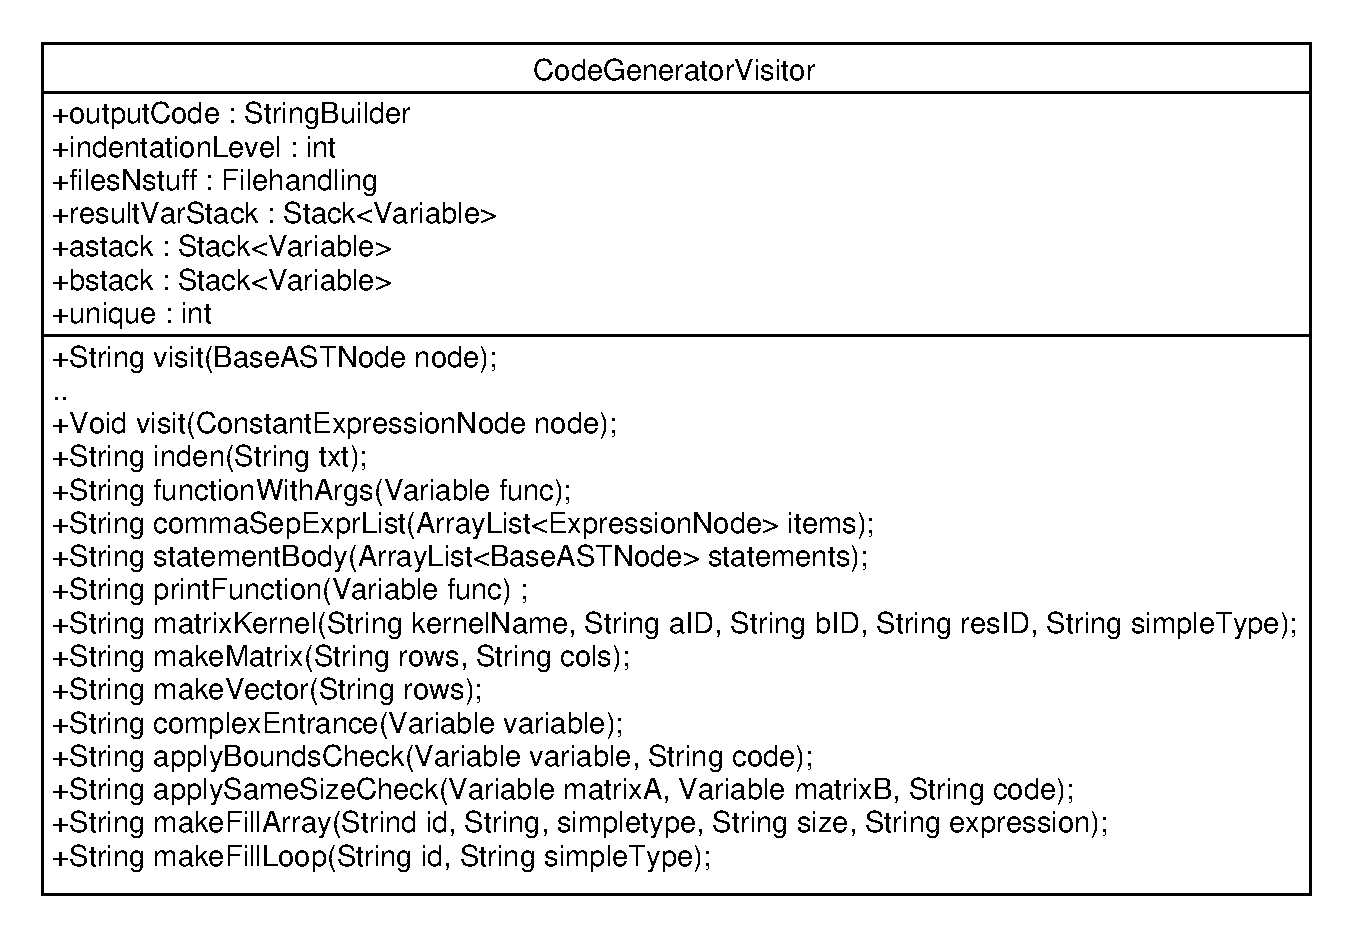
\includegraphics[width=0.8\textwidth]{figures/ClassDiagrams/CodeGeneratorCall.pdf}%trim=4cm 0cm 0cm 0cm, clip
\caption{A class diagram of \texttt{CodeGeneratorVisitor} showing the call from the code generator to the visitor which makes the string from the decorated \acrshort{ast}.}\label{fig:CodeGeneratorVisitor}
\vspace{-15pt}
\end{figure}

The visitor builds a string by traversing the nodes of the tree which will in the end be put into a file by the \texttt{CodeGenerator} class.
Some visit methods like a visit method for a \texttt{ConstantExpressionNode} returns a string while other methods instead directly appends to the string the visitor will return to the class \texttt{CodeGenerator}.
This string is then used as an argument in other visit methods e.g. \texttt{AssignmentNode} which then produces a string which is a statement that can be executed in C.
This string from \texttt{AssignmentNode} is  one of the string to be appended to the string containing the fully compiled program.
%%%%%%%%%%%%%%%%%%%%%%%%%%%%%%%%%%%%%%%%%%%%%%%%%%%%%%%%%%%%%%%%%%%%%%%%%%%%%%%%%%%%%%%%%%%%%%%%%%

As a result the information bubbles upwards from the leafs of the tree to the statementnodes.
The information is put in the correct statementnodes because the visitor pattern makes it possible to specify the route of traversal.
The \texttt{CodeGeneratorVisitor} also contains other methods for producing certain C constructions using the similar \gls{gamble} constructions found in the \acrshort{ast}.
These methods can also be seen on \myref{fig:CodeGeneratorVisitor}.
Some of these methods also make runtime checks of matrices, as matrices needs to be of compatible sizes for some of the operations which can be performed on a matrix, furthermore an index check is implemented such that an out of bounds error will occur if one tries to access memory beyond the bounds of the matrix.
When multiplying two matrices the left matrix of the multiplication has to be a $ N \times M $ while the right one has to be a $ M \times P $ matrix.
So the right matrix must have the same number of columns as the right matrix has rows.
If performing a matrix index multiplication, where every index is multiplied with the corresponding index of the the other matrix, the matrices have to have the same number of rows and columns.

These checks will be inserted as a surrounding if statement around the matrix calculations, so they have to pass these checks before the calculation will be done, if it does not pass an error will be printed.\todo{Der kommer da en fejl right ? - Søren}
The reason this is done at run-time instead of at compile-time is because the sizes of matrices can be dynamic, which results in making it impossible to check for this at compile-time.

When the string is complete it is written to a file called code.c, along with all the other files needed for running the code, e.g. the kernels used for performing computations on the \acrshort{gpu}.
The code.c file is structured so that it is a valid C program.
First off are the libraries included that C uses, then follows a list of prototypes which are all the \gls{gamble} functions translated into C code, both the user made and the ones from libraries.
After the prototypes the main function is made where the body consists of all the statements in the \gls{gamble} sourcecode translated into C.
After the main method all the implementations of the function prototypes are made.
\subsection*{GPU Usage}\label{GPUCode}
Since \gls{gamble} distances its programmers from directly controlling which computations are performed on the \acrshort{gpu}, determing what code to perform on the \acrshort{gpu} becomes a problem for the compiler to solve.\todo{task, lyder bedre eller hvad? MP. - tasks synes jeg ikke rigtigt passer en når det er hvilke kodesegmenter, måske operations hvis det skal ændres? - Marc}
To make this decision the compiler must know what kind of code performs faster on a \acrshort{gpu} than a \acrshort{cpu}.

From \myref{sec:comparch} it is clear that for it to make sense to move any computation to the \acrshort{gpu} it must be of significant size to make up for the overhead of moving data, and be executable in parallel.
If a computation is reliant on the outcome of other computations, the Fibonacci function as an example, moving it to the \acrshort{gpu} would be a significant decrease in performance compared to a \acrshort{cpu}.

Any code written in a recursive format will not be run on the \acrshort{gpu}. 
Furthermore due to the overhead in data transfer, only computations requiring a significant amount of operations to be performed should be executed on the \acrshort{gpu} as \myref{image:benchmark} shows.
Therefore statements which only contain simple data types, i.e. integers, floats and booleans, are performed on the \acrshort{cpu}.
An example could be \texttt{value = value1 + value2}, where all types are integers.
%Therefore statements not containing complex data types, i.e. statements with no vector or matrix arithmetics, are also performed on the \acrshort{gpu}.

However statements that do include matrix or vector arithmetics will be performed on the \acrshort{gpu}.
An example could be matrix multiplication.
Now it is entirely possible to make a matrix multiplication of a $2\times2$ matrix, which would be so small that the overhead of data transfer is more expensive than simply computing on the \acrshort{cpu}. \todo{Det er jo ikke kune data overførslen som koster tid? Der er også JIT af kernel i nogle cases (se alle). -- Troels}
However to simplify the code generation it has been chosen that all matrix or vector calculations, are to be done on the \acrshort{gpu}.
This is not always the best choice, as \myref{sec:comparch} clearly shows, but it requires less analysis of the code given, furthermore as mentioned in \myref{sec:phil} \gls{gamble} uses the \acrshort{gpu} to gain computational power for performing already developed algorithms on data sets big enough to see an improvement in execution time.
Also even if smaller matrices are being computed, the increase in runtime is significantly less than the decrease for just a single bigger matrix operation, as can be seen on \myref{fig:test_results}.
\todo[inline]{Måske nævne vi hellere vil flytte små matricer på gpu, end at beholde store på cpuen? MP - God ide, den tid det tager at flytte en lille matrix til GPU er heller ikke så stor som det man spare på at flytte store matricer til gpu'en. - Søren - Som ovenstående? - Marc}


\subsection*{Runtime Efficiency}\label{subsec:runtime}
A consideration in a compiler is the performance or efficiency of its output. 
Rather than blindly translating the source code, translating to something more efficient is a subproblem in compiler optimisation.\todo{Farlig sætning iflg. Thomas:p - Søren - Men dette er fagtermet, sætningen lige efter specificere dette og nævner også hvorfor det ikke referes til som optimisation fremadrettet, synes den er meget let at komme ud af - Marc}
Optimisation is however a nonspecific and absolute word, therefore in \gls{gamble} we will instead be referring to the problem as improving or increasing runtime efficiency.
Runtime efficiency entails considerations of memory allocation, pipelining, parallelization etc. which may have an impact on execution time.
To do an efficient and complete analysis of how to increase runtime efficiency, information of the situation in a given program is required.
This is where \gls{gamble} is at a disadvantage. 
\gls{gamble} distances its programmers from controlling where the code is performed and instead does so seamlessly.
Information about how e.g. a for-loop could be transformed into a kernel does not exist in \gls{gamble} which makes it difficult to do this.\todo{er ikke helt med her? MP - Vi ved ikke om et for-loop er paralleliser bart eller ej ud fra informationen i AST'et - Marc ... Her kunne en pfor-løkke være brugbar. -- Troels}
The seamless use of the \acrshort{gpu} means that certain information is nonexistent and therefore all computations may not be candidates for improving its runtime efficiency, this is one of the trade-offs \gls{gamble} makes, meaning that simplicity of the language is valued over performance.\todo{Det her står imod principperne og er en farlig og dum sætning tbh. - Søren - Imod hvilke principper? - Marc}
If \gls{gamble} were to require more information, e.g. whether or not something is paralleliseable or ask the programmer to determine what type of \acrshort{gpu} memory should be used for each variable, the simplicity and seamless use of the \acrshort{gpu} would be lost.\todo{Tilføj evt:" and another language like Theano or directly programming OpenCL C might be a better choice." - Søren nb. theano er ikke et sprog -- Troels}

As previously mentioned due to the object code being OpenCL C certain considerations pertaining to instruction handling and register allocation etc. are not of interest for this compiler.
This is handled by using another compiler to compile the OpenCL C code into machine code, see \myref{ssub:makefile}. 
Instead to increase runtime efficiency the considerations concern when the \acrshort{gpu} should be used.\todo{What does this mean? - søren - At fremfor at håndtere performance i forhold til machine code skal det håndteres i forhold til OpenCL C - Marc}

As \gls{gamble} is attempting to seamlessly use the \acrshort{gpu} to increase performance, knowing when the use of the \acrshort{gpu} will actually be beneficial is an important point in the code generation process. \todo{Kom pludselig til at tænke på det jo ikke er vores sprog der bruger gpu'en men blot vores compiler der gør at vi gør det? Er det så forkert at skrive som her ? - Søren - Men det er som følge af vores sprog at det er seamless? kan ikke helt se hvad du vil skrive som alternativt, eller hvorfor det skulle være forkert - Marc}
As mentioned to do this efficiently, the compiler would require more information about the computations in a \gls{gamble} program than can be read from the syntax of \gls{gamble}.
Therefore it is decided that it is better to be sure that a computation can benefit from the \acrshort{gpu}, rather than risking moving computations that wont benefit with those that will.
As such only the operations that the project group knows have a possibility of benefiting from the parallel computational power of the \acrshort{gpu} will be executed on the \acrshort{gpu}.

%Knowing when to use GPU
Even though a computation can be parallelised, it does not necessarily mean it should be moved to the \acrshort{gpu}, as is evident in \myref{image:benchmark}.
This is an opportune moment for improving the runtime efficiency of the object code by using the \acrshort{gpu} only when it will be superior to the \acrshort{cpu} in regards to performance.
A possibility of doing so would be to analyse whether or not an instruction sequence both entail a sufficient amount of operations and that these are not sequentially dependent on each other.
Performing such an analysis increases compile time.
Because of the difficulty to discern not only if there will be an actual increase, but also if any custom functions created by a programmer are fit to be run on the \acrshort{gpu} this analysis is not part of the compiler.
Instead only vector and matrix operations already defined in the language, by having a special operator assigned to them, will be performed on the \acrshort{gpu}.

%Optimising OpenCL Kernals
A function that is to be run on the \acrshort{gpu} is in the OpenCL framework called a kernel.\todo{er nævnt før. MP}
Since kernel code uses explicit memory handling, one must choose what memory space on the \acrshort{gpu} to allocate ones variables in as well as using the principle of locality.
This can provide a substantial (more than 3 times) faster runtime. \citep{ocl_lecture3}
\begin{figure}[h]
\centering	
 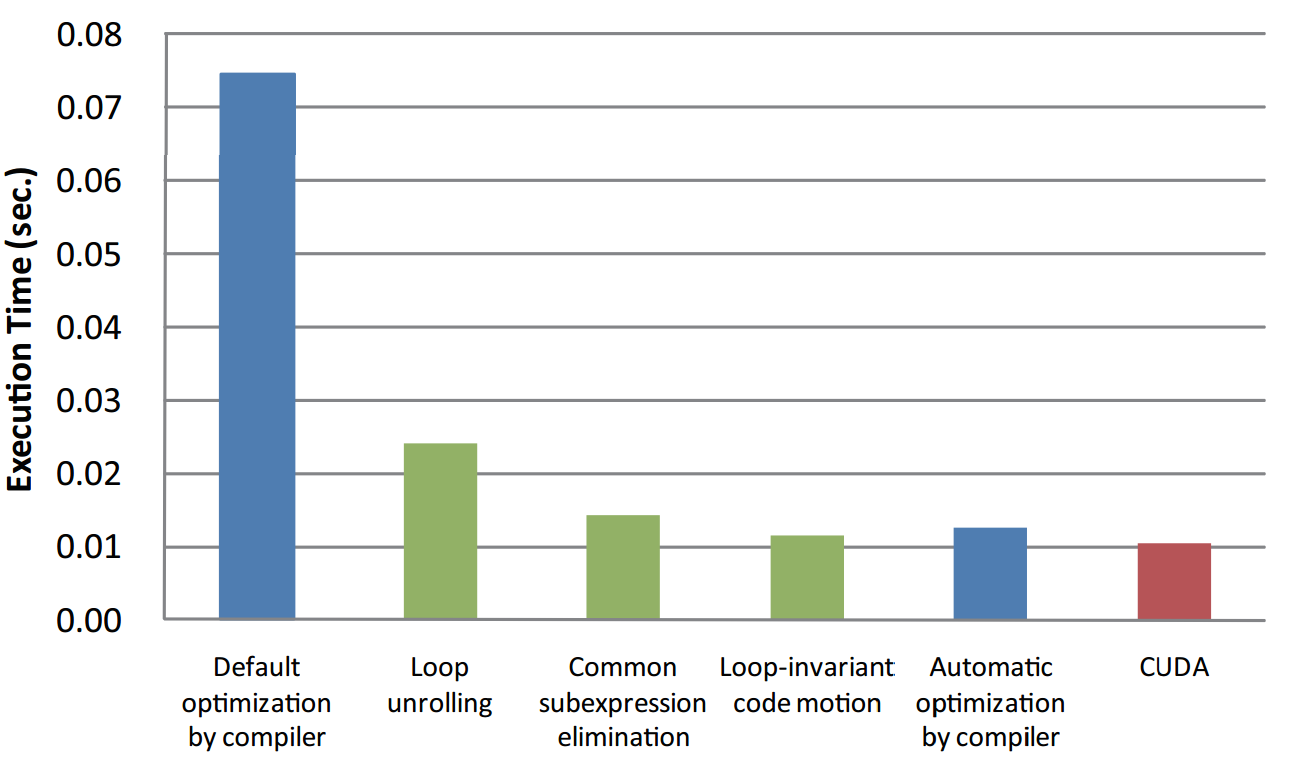
\includegraphics[width=1\textwidth]{figures/opencloptimisation.png} % trim=4.85cm 15cm 0.85cm 1cm
\caption{Execution speed of a matrix multiplication with different increases in runtime efficiency done. \todo[inline]{Det ville være TRIVIELT at forklare hvad disse optimeringer er og hvorfor programmet er hurtere på grund af det. Skal vi det? -- Troels} \citep{CUDAOpenCLOptimisation}}\label{image:OpenCLOptCompare}
\vspace{-15pt}
\end{figure}
\todo[inline]{dette er plagiat. Det skal tydeligt fremgå det ikke er vores billede. MP - Det fremgår da også rimelig tydeligt i det at der er en kilde på billedet? - Marc}
As seen on \myref{image:OpenCLOptCompare} some possible methods of increasing runtime efficiency includes loop unrolling, common sub-expression elimination and loop-invariant code motion. 
These are taken as specific examples in this comparison because these methods are performed in the \acrfull{ptx} code that CUDA compiles to. %ENDING A SENTENCE WITH A PROPOSITION OMG!!!
An OpenCL C compiler will also increases the runtime efficiency of the source code if given the instruction to, however its impact depends on the \acrshort{gpu} and platform in use.
The value of any increases in runtime efficiency is situational, i.e. changing the work-group size can yield improvements of up to 5 times. \citep{ocl_lecture3}
OpenCL can use \acrshort{jit} to generate binary code to the appropriate device it is working with at runtime.
This allows OpenCL to increases in runtime efficiency for the \acrshort{gpu} used, however this is also a constant overhead for each execution of the program. 
OpenCL can also compile the kernels before runtime, this is known as an offline compilation as opposed to the \acrshort{jit} compilation known as online compilation. 
The CUDA compiler \texttt{nvcc} is a two step process, which first generates \acrshort{ptx} bytecode and then either \acrshort{jit} compile on runtime or compiles a so called ``fat binary''at compile time, which contains multiple programs for different \acrshort{gpu}s. \citep{nvidia_cude_fat_bin}

%Optimising C code(CPU)
As \gls{gamble} does not exclusively perform its operations on the \acrshort{gpu} the code run on the \acrshort{cpu} must also be considered as a point in which runtime efficiency can be increased.
Some methods of increasing runtime efficiency on the \acrshort{cpu} are similar as mentioned earlier such as loop unrolling.\todo{Skal vi evt. forklare hvad det er ?? - Søren Er enig, men måske er det for trivielt? At forklare det vil dog vise vores kendskab til det. -- Troels}
Further methods pertain to the architectural differences between \acrshort{cpu}s and \acrshort{gpu}s, in particular cache- and pipeline-friendly code.
Cache-friendly code means considering the principle of spatial locality i.e. memory regions closer to each other, are more likely to be accessed within a short time.
To write pipeline-friendly code one must in particular consider branch prediction, however the best way is simply to avoid branching. \citep{CCodeOpt}
While these methods may very well increase runtime efficiency, there is no reason to implement them as the GNU Compiler Collection (GCC) already implements well developed methods of increasing runtime efficiency beyond our abilities.
\section{Implementation}
This section will show examples from the compiler code which generates the object code from the source code in \gls{gamble}.
This will show an implementation of several design choices made in the previous chapters.
First an example of how a \texttt{DeclarationNode} is translated into C code will be provided; afterwards the implementation of using the \acrshort{gpu} using OpenCL will be presented.
The compiler starts the codegeneration by calling an instance of the class \texttt{CodeGenerator} and invoking the method \texttt{GenerateCodeAndWriteToFile}.
This method then makes the \acrshort{ast} accept a CodeGeneratorVisitor and writes its output to a file; while also exporting the object code to a certain directory along with other files needed; the OpenCL kernels used in the program.
The \texttt{outputCode} is a string which starts as an empty string; every visitor then either appends or returns substrings to be appended.
These substrings add different information to the \texttt{outputCode} string as the traversal is ongoing.
\begin{figure}
\centering
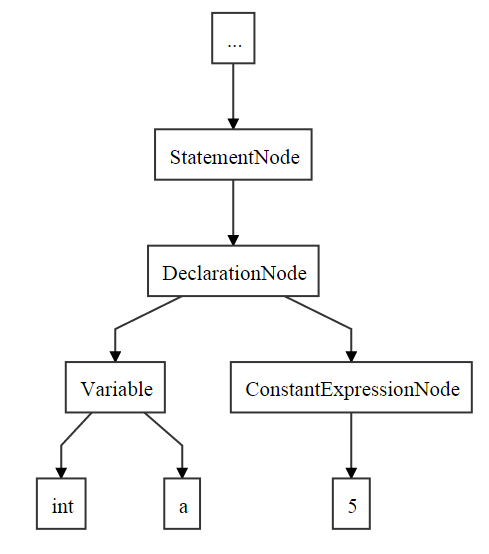
\includegraphics[width=0.5\textwidth]{figures/Trees/ASTAlone.PNG}
\caption{An \acrshort{ast} for the declaration \texttt{int a = 5;}}\label{fig:ASTAlone}
\end{figure}

\myref{fig:ASTAlone} shows a \texttt{DeclarationNode} for the expression \texttt{int a = 5;}. 
In the code generator this node will be transformed into the declaration written in C. 
The syntax for this is actually the same in C as it is in \gls{gamble}. 
The node has been through the previous phases, type and scope check, and is therefore ready to be computed.
The code executed when the visitor accepts a \texttt{DeclarationNode} can be seen on \myref{lst:DeclarationNodeCodeGen}.
\begin{lstlisting}[float, floatplacement=H!, caption=The visit method for visitting a DeclarationNode in the codegenerator. ,frame=tlrb,label={lst:DeclarationNodeCodeGen}]
@Override
public String VisitDeclarationNode(DeclarationNode node) {
    String expr = "";
    String complexType = "";
    if (node.getExpression() != null){
        resultVarStack.push(node.getVariable());
        expr = visit(node.getExpression());
        resultVarStack.pop();
    }

    if (node.getVariable().isComplex()) {
        ...
    }
    if (expr.indexOf("sclManageArgsLaunchKernel
    	(hardware, software, global_size, local_size") >= 0){
        ...
    }
    
    return complexType.length() > 0 ? complexType + expr : 
    (node.getVariable().toCcode() + " = " + expr + ";");
}
\end{lstlisting}
Since the example \texttt{int a = 5;} is not of a complex data type like a matrix or vector the body of the second and third if statements are hidden.\todo{Måske vise den i bilag hvor den ikke er hidden?}
A method is called on the node to check whether the expression that assigned the declared variable exists. 
Syntactically a matrix or vector may appear to be uninitialised but this actually creates a vector or matrix filled with zeros.
In \myref{lst:DeclarationNodeCodeGen} the expression is not null so it enters the body of the \texttt{if} statement on line 5.
The result variable, which stores the result of the expression, is pushed to a stack before visiting the expression.
In the method \texttt{VisitExpresssionNode} the top of the stack, which the result was pushed to, is checked to see if the result is a complex datatype or not; in the example the result is not of a complex data type and the expression is then evaluated by visiting the nodes of the expression.
The result of the call to \texttt{VisitExpressionNode} is saved to a string \texttt{expr}.
Another if statement checks if the declaration needs a kernel and if the expression needs to be computed on the \acrshort{gpu}.
When the call to \texttt{VisitDeclarationNode} returns; it is checked whether the string \texttt{complexType} has been made longer or not.
In the example \texttt{int a = 5;} it has not and therefore the string of the datatype and ID are concatenated with the assignment symbol, the substring \texttt{expr} and a semi-colon, before finally being returned.






In the following section an introduction of a library called SimpleOpenCL will take place.
\subsubsection*{Using SimpleOpenCl}
Simple\gls{opencl} is a library for C which simplifies the process of setting up and launching a kernel for \gls{opencl}.
The kernels remain the same, but finding the hardware for executing the kernels and allocating memory for the hardware is simplified.

The \texttt{CodeGeneraterVisitor} starts at the root of the \acrshort{ast} and here the code on \myref{lst:OpenCLSetup} is run.

\begin{lstlisting}[caption=Call to setup Simple\gls{opencl} in the compiler by appending it to a string builder,numbers=none,frame=tlrb,label={lst:OpenCLSetup}]
outputCode.append(filesNstuff.
	 ImportStringFromResource("codesnippets/simpleCLsetup.c") + "\n\n");
\end{lstlisting}
The file simpleCLsetup.c is appended to the code right as the main method of the output file is started.
The file contains the code which can be seen on \myref{lst:OpenCLSetup2}.

\begin{lstlisting}[caption=Simple\gls{opencl} setup in the compiler,numbers=none,frame=tlrb,label={lst:OpenCLSetup2}]
// Simple-\gls{opencl} Hardware setup
	sclHard* allHardware;
	sclHard hardware;
	sclSoft software;
	int found = 0;
	allHardware = sclGetAllHardware( &found );
	hardware = sclGetFastestDevice(allHardware, found);

    size_t local_size[2] = {1, 1};
    size_t global_size[2] = {1, 1}; 

    printf("\n");
// END Hardware setup
\end{lstlisting}

This code creates the elements needed to launch a kernel.
It finds the fastest hardware according to SimpleOpenCl's function calls, which means it finds the device with the most number of compute units, no matter the type of device, be it a \acrshort{cpu} or a \acrshort{gpu}.
For the remaining part of this section the fastest device is a \acrshort{gpu}.
\texttt{global\_size} and \texttt{local\_size} are there to determine the amount of memory needed both globally and locally on the \acrshort{gpu}.
The size of these arrays are initialised to two, because the \gls{gamble} matrices are two-dimensional.
These arrays are then filled out with different numbers corresponding to the columns and rows of the matrices or vectors being calculated upon.
This way of appending templates to the outputCode string is used in different places in the code generation when handling the complex datatypes matrices and vectors.
In fact whenever one of the following operators \texttt{+, -, *, \#, \^{} } are used with matrices or vectors a template is being appended to the outputCode. 
See \myref{tbl:matOps} for a description of what each operator will produce in \gls{gamble}.

When the right side of an assignment or declaration consists of an expression using operators and matrices or vectors, the visitor checks which operator is used and then inputs a template for launching the kernel depending on the operator.
The compiler contains files which have the code for launching the kernel for the specific situation and also for the kernel itself.
If a kernel is used the kernel file is added to the ``codeout'' directory along with the output code itself.

\myref{lst:kernelLaunch} shows one of the kernels being appended to the outputCode.

\begin{lstlisting}[caption=Simple\gls{opencl} launch of a kernel calculating a matrix or vector multiplied with a scalar.,numbers=none,frame=tlrb,label={lst:kernelLaunch}]
//MATRIX §MATRIX_A§ MULTIPLIED WITH A SCALAR §MATRIX_B§
global_size[0] = §MATRIX_A§.rows*§MATRIX_A§.cols;
local_size[0] = 1;
global_size[1] = 1;
local_size[1] = 1;
software = sclGetCLSoftware("matrixMulScalar.cl", "matrixMulScalar", hardware);
§MATRIXTYPE§ scl_scalar_mul§NUM§ = §MATRIX_B§;
// %R means that what is being sent can be read from and written to
// %a means that what is being sent is a non-pointer argument and is constant
sclManageArgsLaunchKernel(hardware, software, global_size, local_size, "%R %a",
    §MATRIX_A§.dataSize, §MATRIX_A§.dataStart, sizeof(§MATRIXTYPE§), &scl_scalar_mul§NUM§);
//END MATRIX SCALAR MULTIPLY
\end{lstlisting}

\texttt{global\_size} is set to be the size of the matrix, and a kernel is then launched for every index in the matrix.
This is decided by setting the indices in \texttt{global\_size}.
If the squared matrix was 2x2, a kernel would be launched with 0, 1, 2 and 3 as the indices.
The implementation of multiplying a matrix with a scalar is made where the matrix is interpreted as a single vector where each row comes after the other.
If the matrix form is needed the rows of the matrix would be placed in \texttt{global\_size[0]} and the columns in \texttt{global\_size[1]}.
If the example of a size 4 matrix is still used, the following sets of kernels would be sent:
\begin{equation}
\{0,0\}, \{0,1\}, \{1,0\}, \{1,1\}
\end{equation}
So a kernel for each index in the matrix.
This can then be used in the kernel to determine which row and which column, the index being sent to the kernel for execution, possess.
The \texttt{software} is where the kernel being launched is set, the file name and the kernel name in the file, the hardware for the execution must also be set.
Then the function \texttt{sclManageArgsLaunchKernel()} handles the launching itself with the variables needed to launch the kernel.
Before this code is appended any string with  \S-signs is is replaced by the corresponding string depending on the situation.
So \texttt{§MATRIX\_A§} is replaced with the id of the left matrix in the expression node.
The code for replacing the strings can be seen on \myref{lst:replaceString}.

\begin{lstlisting}[caption=Code for replacing strings with the corresponding information to be appended to the outputCode.,numbers=none,frame=tlrb,label={lst:replaceString}]
private String matrixKernel(String kernelName, String aID, String bID, String resID, String simpleType) {
    String kernel = filesNstuff.ImportStringFromResource("kernels/" + kernelName + ".cl");
    kernel = kernel.replaceAll("§MATRIXTYPE§", simpleType);
    filesNstuff.WriteToFile(new File("../../../codeout/" + kernelName + ".cl"), kernel);

    String argsNlauch = filesNstuff.ImportStringFromResource("kernelLaunch/" + kernelName + ".c");
    argsNlauch = argsNlauch.replaceAll("§MATRIX_A§", aID);
    argsNlauch = argsNlauch.replaceAll("§MATRIX_B§", bID);
    argsNlauch = argsNlauch.replaceAll("§MATRIX_RES§", resID);
    argsNlauch = argsNlauch.replaceAll("§MATRIXTYPE§", simpleType);
    argsNlauch = argsNlauch.replaceAll("§NUM§", Integer.toString(this.scalarNum));
    argsNlauch = argsNlauch.replaceAll("\\n", "\n" + indent(""));
    return argsNlauch;
}
\end{lstlisting}

However this must also be done for the kernel itself, in the kernels the type is changed depending on the type of the fields in the matrix or vector, which makes it possible to use the same code in the code generator for replacing these strings, since the type is handled dynamically.

The corresponding kernel for \myref{lst:kernelLaunch} can be seen on \myref{lst:kernel}.
\begin{lstlisting}[caption=Kernel code for multiplying a matrix or vector with a scalar.,numbers=none,frame=tlrb,label={lst:kernel}]
__kernel void matrixMulScalar(__global §MATRIXTYPE§ *ma, §MATRIXTYPE§ scalar){
	int global_x = get_global_id( 0);
	ma[ global_x] *=  scalar;
}
\end{lstlisting}

As can be seen the string \texttt{§MATRIXTYPE§} must also be replaced here.
The index which has been sent to the kernel is retrieved by calling \texttt{get\_global\_id(0);}.
The index is then used to access the matrix at the specific index and multiply the value at the index with the scalar.


\subsubsection*{From OpenCL to execution}\label{makefile}
After the \gls{gamble} compiler have compiled the source code; the compiler outputs OpenCL C code as its object code.
The OpenCL C code must be compiled by a C-compiler such as the GCC (GNU Compiler Collection) compiler to produce code the \acrshort{cpu} and \acrshort{gpu} can execute.
During the compilation the OpenCL C headers must be accessable, to provide the functions and types used. 
Aditionally the \gls{gamble} standard libary, containing functions such as \texttt{matrixToFile} and \texttt{fileToMatrix} must also be included and compiled. 
This produces an executable file for the platform targetted by the compiler, this will most often be the platform running, such as x86--64 on Linux.
The same executeable file is not usable for another platform, e.g. ARM, nor on another operating system, e.g. Windows or OS X.\todo{Skal vi ændre dette til OS X only med gamble?}
To maintain portability a ``MakeFile'' is used; a MakeFile is a file in the syntax which the GNU make utility can execute. 
The make utiliry is a set of rules which ensures that the correct compiler, path, headers, etc. are used during compilation on one of multiple platforms. 
This means that after running the \gls{gamble} compiler, on a configured computer, e.g. has OpenCL C headers, libary, a compiler etc., the make command can be used to build a binary file to be executed.

The kernel can either be compiled at compile-time or \acrshort{jit} compiled at runtime.
The JIT compilation, called online compilation under OpenCL, allows the system to adapt with platform specific optimisations for the running platform.
If the kernel is compiled at compile-time, called offline compilation under OpenCL, then it might support fewer devices, or will take a long time and increase the size of the executable as it has to contain versions for each hardware for which support is requested. \citep{openclbookjit}
For \gls{gamble} the online compilation is chosen for its simplicity as it lets the driver of the running system compile the kernel. 

A typical compilation on Ubuntu 14.04 configured with OpenCL headers located at \path{/opt/opencl-headers/include/} will look like \myref{lst:makecommands}, where \texttt{code.c} is the output of the \gls{gamble} compiler.
After the execution of these, an output file called \texttt{run} is made and can be executed with the command \texttt{./run}. 

\begin{lstlisting}[caption=The commands executed by the make command according to the rules of the MakeFile,numbers=none,frame=tlrb,label={lst:makecommands}]
gcc -Wall -Wextra -pedantic -O3 -std=c99 -I/opt/opencl-headers/include/ -c code.c simpleCL.c gambleStdlib.c
gcc -Wall -Wextra -pedantic -O3 -std=c99 *.o -o run -lm -lOpenCL -lrt
rm -f *.o
\end{lstlisting}
